%% Based on a TeXnicCenter-Template by Gyorgy SZEIDL.
%%%%%%%%%%%%%%%%%%%%%%%%%%%%%%%%%%%%%%%%%%%%%%%%%%%%%%%%%%%%%
%
%------------------------------------------------------------
%
\documentclass[a4paper,12pt,reqno]{article}
%----------------------------------------------------------
\usepackage{amsfonts}
\usepackage{listings}
\usepackage{graphicx}
\usepackage{geometry}
\usepackage{xcolor}
\usepackage{amssymb,amsmath}
\usepackage{polski}
\usepackage[T1]{fontenc}
\usepackage[utf8]{inputenc}
\usepackage{caption}
\geometry{margin=1.1in}
\usepackage{wrapfig}
\usepackage{lipsum}  
\usepackage{listings}
\usepackage[toc,page]{appendix}
\usepackage{url}
\usepackage{float}
\usepackage{amsmath}
\usepackage{indentfirst} % pierwszy akapit zawsze z wcięciem
\usepackage{subcaption}	% kilka zdjęc w jednej lini
\usepackage{blindtext}
\usepackage[hidelinks]{hyperref}
\definecolor{codegreen}{rgb}{0.5, 0.09, 0.09}
\definecolor{codegray}{rgb}{0.5,0.5,0.5}
\definecolor{codepurple}{rgb}{0.58,0,0.82}
\definecolor{backcolour}{rgb}{0.94,0.94,0.94}
\definecolor{gray}{rgb}{0,0.6,0}

\lstdefinestyle{mystyle}{
    backgroundcolor=\color{backcolour},  
    commentstyle=\color{codegreen},
    keywordstyle=\color{blue},
    numberstyle=\tiny\color{codegray},
    stringstyle=\color{codepurple},
	basicstyle=\footnotesize\fontfamily{cmtt}\selectfont,
    breakatwhitespace=false,         
    breaklines=true,
    captionpos=b,
	language=C++,
    keepspaces=true,                 
    numbers=left,                    
    numbersep=5pt,                  
    showspaces=false,                
    showstringspaces=false,
    showtabs=false,                  
    tabsize=2
}

\lstset{style=mystyle}
\lstset{literate=%
    *{0}{{{\color{gray}0}}}1
    {1}{{{\color{gray}1}}}1
    {2}{{{\color{gray}2}}}1
    {3}{{{\color{gray}3}}}1
    {4}{{{\color{gray}4}}}1
    {5}{{{\color{gray}5}}}1
    {6}{{{\color{gray}6}}}1
    {7}{{{\color{gray}7}}}1
    {8}{{{\color{gray}8}}}1
    {9}{{{\color{gray}9}}}1
}
\lstset { %
    language=C++,
    backgroundcolor=\color{black!5}, % set backgroundcolor
    basicstyle=\footnotesize,% basic font setting
}
%------------------------------------------------------------
\begin{document}

%\begin{figure}[h]
%	\centering
%		
\includegraphics[width=0.40\textwidth]{logo.pdf}
%\end{figure}


\begin{center}

\thispagestyle{empty}

%UNIWERSYTET WROCŁAWSKI\\
\Large 
Uniwersytet Wrocławski\\
Wydział Fizyki i Astronomii\\
\vspace{0.8cm}
\vspace{1.8cm}

\Large Marcin Pietrzak \\
\vspace{3.2cm}
\Large Galeria modeli komputerowych w silniku Unreal \\
\vspace{1.5cm}
Computer models gallery in Unreal Engine
\end{center}
\vspace{3.7cm}
\begin{flushright}

\large{ Praca inżynierska na kierunku \\Informatyka Stosowana i Systemy Pomiarowe \\}
\vspace{0.5cm}
\large{ Opiekun \\ dr hab. Maciej Matyka, prof. UWr}
\end{flushright}
\vspace{2.2cm}

\begin{center}
\large Wrocław, \today
\end{center}

\newpage

\tableofcontents

\newpage

\begin{flushleft}
\Large \textbf{Streszczenie}
\end{flushleft}
\vspace{1cm}


 Lorem ipsum dolor sit amet, consectetur adipiscing elit, sed do eiusmod tempor incididunt ut labore et dolore magna aliqua. Ut enim ad minim veniam, quis nostrud exercitation ullamco laboris nisi ut aliquip ex ea commodo consequat. Duis aute irure dolor in reprehenderit in voluptate velit esse cillum dolore eu fugiat nulla pariatur. Excepteur sint occaecat cupidatat non proident, sunt in culpa qui officia deserunt mollit anim id est laborum.

\newpage
\begin{flushleft}
\Large \textbf{Abstract}
\end{flushleft}
\vspace{1cm}


Lorem ipsum dolor sit amet, consectetur adipiscing elit, sed do eiusmod tempor incididunt ut labore et dolore magna aliqua. Ut enim ad minim veniam, quis nostrud exercitation ullamco laboris nisi ut aliquip ex ea commodo consequat. Duis aute irure dolor in reprehenderit in voluptate velit esse cillum dolore eu fugiat nulla pariatur.

\newpage

\section{Wstęp}

\subsection{Wprowadzenie}

W ciągu ostatnich 10 lat rynek gogli VR zaczął się budzić na nowo dzięki jednemu z ojców założycieli firmy Oculus, Palmer Luckey. Wieku 16 lat zaczął budować swoje pierwsze gogle VR, a kilka lat później założył firmę Oculus i dzięki udanej zbiórce na Kickstarterze jego firma miała fundusze stworzyć swoje pierwsze sklepowe gogle. Po drodze firma wypuściła kilka prototypów dla deweloperów. Sama firma została przejęta przez Facebooka, dzisiaj znana jako Meta, za 2 miliardy dolarów w 2014 roku. Ich pierwsze komercyjne gogle, Oculus Rift, zostały wydane w 2016 roku i kosztowały na start 599 dolarów. W 2017 roku z firmą pożegnał się Palmer Luckey, który obecnie zajmuje się firmą tworzącą technologię obronne. Natomiast kolejnym komercyjnym sprzętem Oculusa był Oculus Go wydanym w 2018 roku jako sprzęt all-in-one, czyli nie wymagały zewnętrznych urządzeń, czy przewodów do działania. Gogle dzięki brakowi potrzeby podłączania komputera, czy smartfonu okazały się ogromną innowacją na rynku sprzętu VR. Koszt gogli zaczynał się od 199 dolarów w dniu premiery. W kolejnym roku zostały wydane dwa nowe rodzaje gogli. Pierwszym był następca Oculusa Rifta, czyli Oculus Rift S kosztującym 400 dolarów. Podobnie jak jego poprzednik były stworzone zmyślą o PCVR. Recenzentom sprzęt też nie przypadł do gustu, zarzucając mu zbyt małą ilość innowacji od poprzedniej wersji. Inaczej było z drugim produktem, który wypuścili w podobnym czasie, czyli Oculus Quest. Cena premierowa zaczynała się od 399 dolarów. Quest, podobnie jak jego poprzednik nie wymagał żadnych dodatkowych urządzeń do działania. Dzięki dość niskiej cenie, jak za możliwości, które oferowały gogle, okazały się one ogromnym sukcesem dla Oculusa na tyle ogromnym, że zaczęły one powoli wypychać swojego brata Rift S z rynku, a gwoździem do trumny dla Rift S było ogłoszenie przez Oculusa, że można będzie Questa podłączyć do PC i korzystać z nich jak Rift S. Sam Oculus od tego momentu zaczął tworzyć tylko gogle autonomiczne.

\begin{figure}[!ht]%
	\centering
	\begin{subfigure}{.5\textwidth}
		\centering
		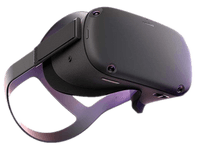
\includegraphics[width=0.8\linewidth]{graphics/oculusquest.png}
		\caption{Oculus Quest 1}	
		\label{ref:subref_a}
	\end{subfigure}%
	\begin{subfigure}{.5\textwidth}
		\centering
		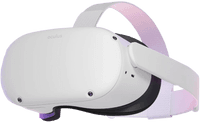
\includegraphics[width=0.8\linewidth]{graphics/oculusquest2.png}
		\caption{Meta Quest 2}
		\label{ref:subref_b}
	\end{subfigure}%
	

\caption{Gogle VR od Reality Labs.}
\label{ref:ref}
\end{figure}


W kolejnym roku, tj. 2020 wypuścili kolejne gogle, czyli Oculus Quest 2, których koszt zaczynał się od 299 dolarów. Dzięki jeszcze niższej cenie i lepszej mocy w stosunku do poprzednika stały się najpopularniejszymi goglami na rynku. W ciągu ostatnich dwóch lat Oculus zmienił nazwę na Reality Labs, Facebook na Meta, a Oculus Quest 2 na Meta Quest 2. Obecnie Meta jest firmą próbującą stworzyć swój pierwszy metavers. W ostatnich tygodniach wypuścili też gogle z myślą o zastosowaniach biznesowym i dla metaversum, Meta Quest Pro kosztujące 1500 dolarów. Oczywiście same gogle Meta nie są jedyne na rynku. Podczas boomu na rynku VR w 2016 zostały wydane też inne gogle konkurencyjnych firm. Do największych należą HTC Vive, gogle wydane przez HTC we współpracy z firmą Valve, jako główny konkurent Oculus Rifta, bo podobnie jak Rift też były tworzone z myślą o rynku PC. Trochę inną drogo poszło Sony, tworząc PlayStation VR, były to gogle stworzone z myślą o konsoli PlayStation 4. Natomiast w latach 2016-2022 powstała co najmniej setka nowych gogli VR różnych firm \cite{ilosc_urzadzen}, z czego największą popularnością są gogle od Mety \cite{popularnosc_gogli}, w 2021 roku zostało sprzedanych 11 milionów sztuk urządzeń, z czego 78\% były to Meta Quest 2 \cite{ilosc_urzadzen}.

\begin{figure}[!ht]%
\centering
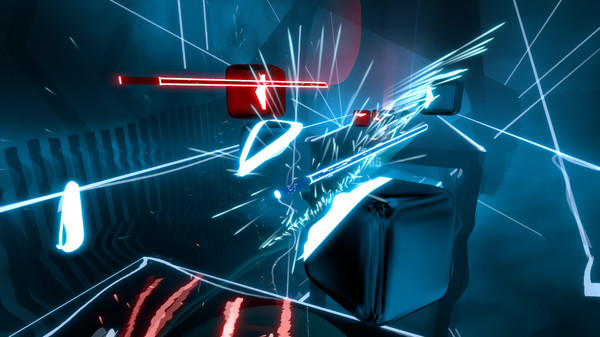
\includegraphics[width=0.8\columnwidth]{graphics/BeatSaber.jpg}
\caption{Przykład gry stworzonej z myślą o VR: "Beat Saber" firmy Beat Games.
\label{OpenBrush}}%
%
\qquad
\end{figure}  


Rynek aplikacji VR też się rozwinął w ciągu ostatnich lat. Producenci silników gier, tacy jak Epic czy Unity dodali wsparcie gogli wirtualnej rzeczywistości. Dzięki wparciu od dużych firm rozpoczął się wysyp różnego rodzaju aplikacji. W oficjalnym sklepie Oculus jest obecnie dostępnych ponad 400 aplikacji \cite{liczba_gier_quest}, na Steam jest ich już ponad 4000 \cite{liczba_gier_steam}. Oczywiście sam sprzęt nie służy też do rozrywki. Może być też wykorzystywany np. przez wojsko do tworzenia symulacji, czy przez artystów do tworzenia dzieł sztuki lub galerii modelów komputerowych.

\subsection{Cel i zakres pracy}

Głównym założeniem pracy jest stworzenie aplikacji VR, która przedstawi kilka wybranych modeli komputerowych. Dodatkowo będą znajdować się tam informację o modelu w formie galerii, w której znajdować się będzie historia danego modelu i ciekawostki z nim związane. Użyte gogle VR do pomocy przy tworzeniu aplikacji to Oculus Quest. Aplikacja została natomiast napisana w silniku Unreal Engine oraz w środowisku programistycznym Visual Studio 2022. Silnik UE4 posiada wsparcia dla gogli VR, a także można w nim pisać klasy i skrypty w języku C++ oraz przy wykorzystaniu Blueprintów. Jest to wizualny język skryptowy stworzony z myślą o ludziach, którzy nie mieli styczności z językiem programowania, np. dla game designerów, którzy mogą zrobić proste skrypty, a następnie programista może je przerobić na skrypty C++. Dodatkowo po stronie C++ można stworzyć bazowy system, który może zostać rozszerzony w Blueprintach o funkcje, do których dostęp jest łatwiejszy w Blueprintach. Celem niniejszej pracy, jest pokazanie, że przy dzisiejszej technologii i wiedzy można stworzyć program w sposób, który nie byłby możliwy do zrealizowania jeszcze 10 lat temu.

\begin{figure}[!ht]%
\centering
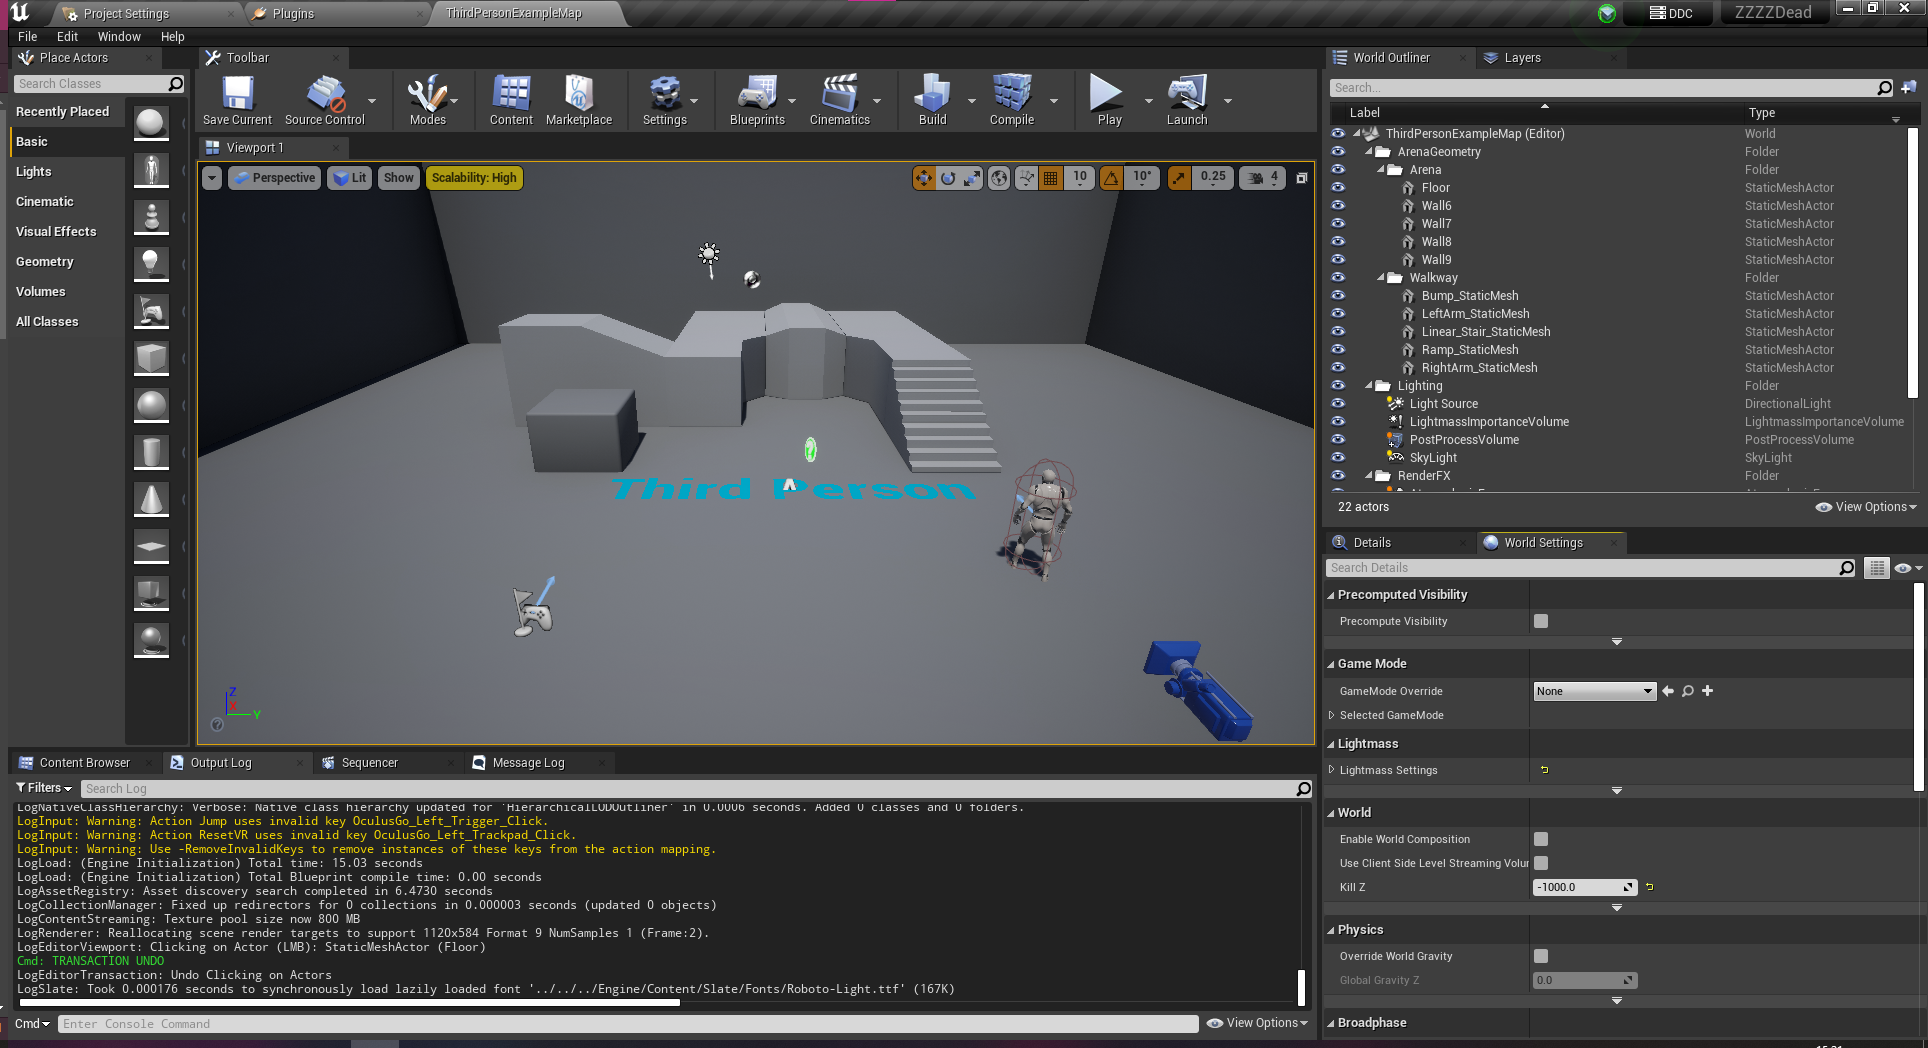
\includegraphics[width=1\columnwidth]{graphics/UE4View.png}
\caption{Podstawowy wygląd programu Unreal Engine 4.
\label{OpenBrush}}%
%
\qquad
\end{figure}  

\begin{figure}[!ht]%
\centering
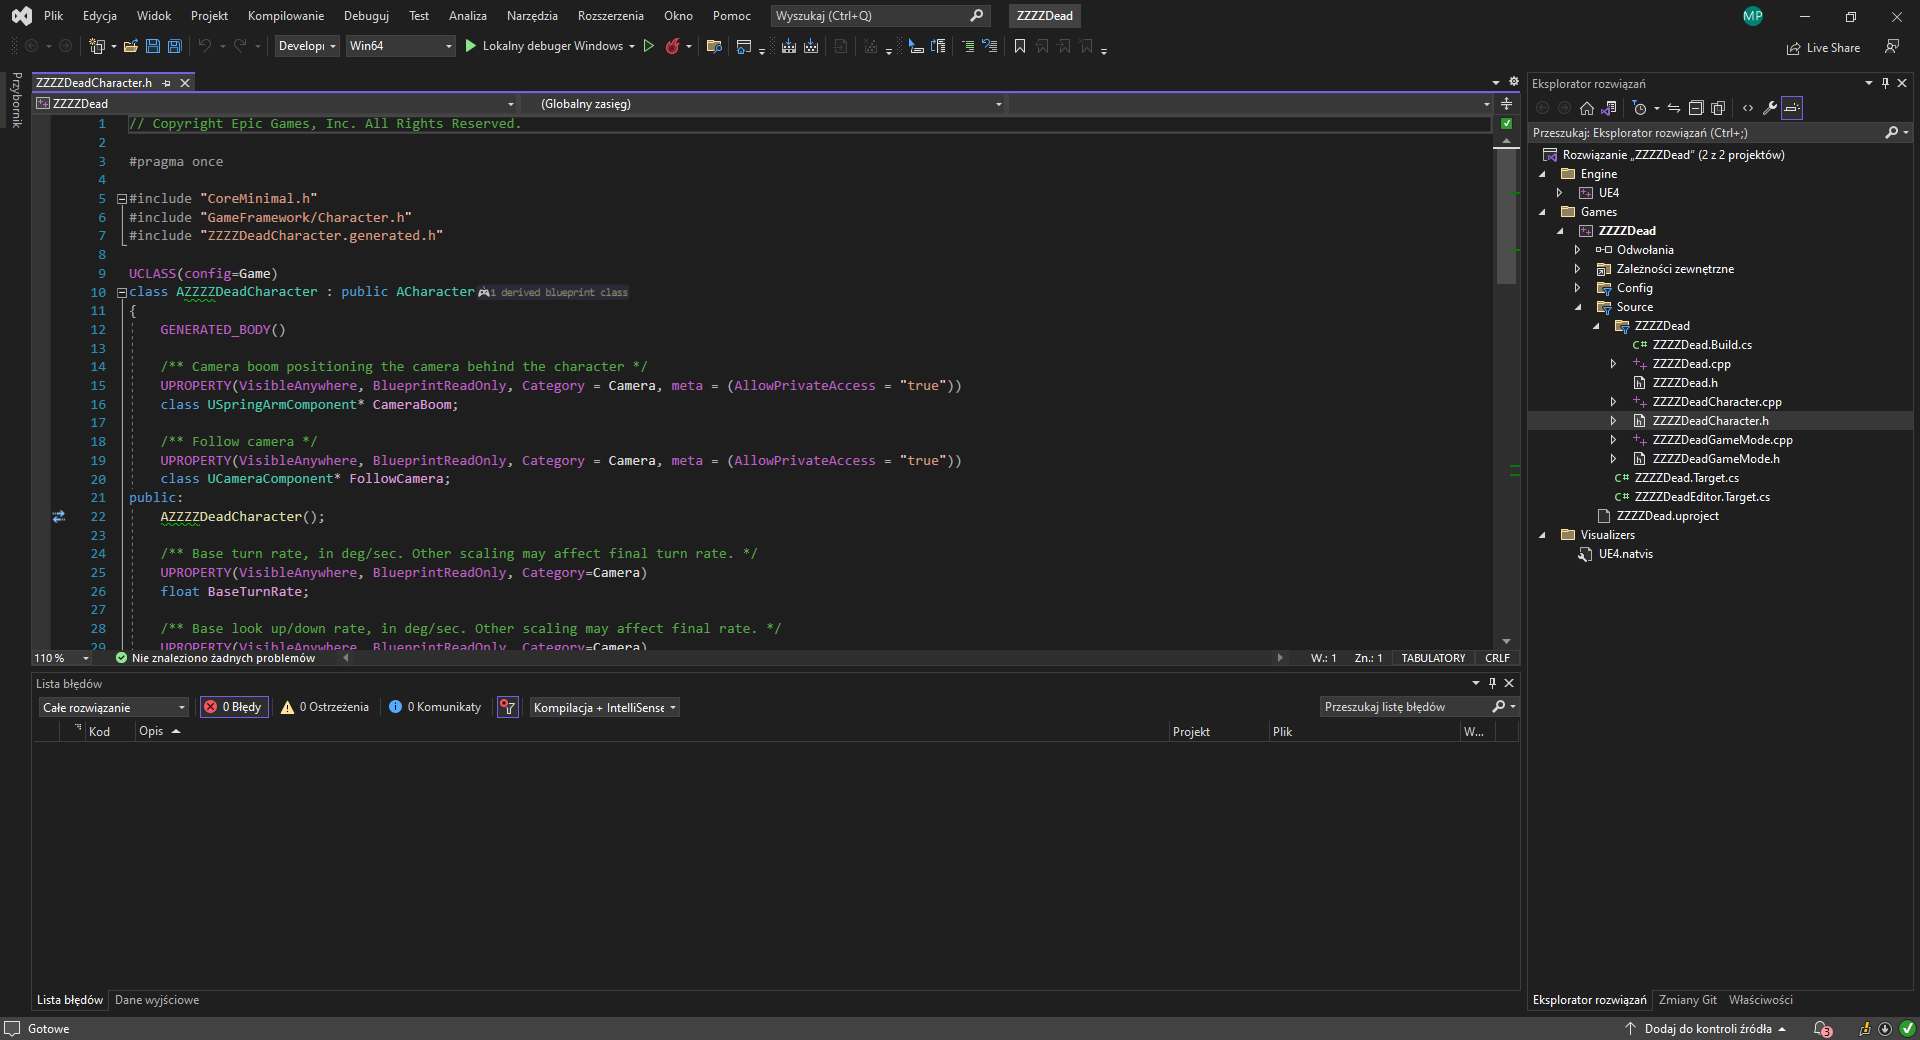
\includegraphics[width=1\columnwidth]{graphics/VSView.png}
\caption{Podstawowy wygląd programu Visual Studio 2022.
\label{OpenBrush}}%
%
\qquad
\end{figure}  

\newpage
\section{Warstwa Użytkowa}

\subsection{Wygląd i Obsługa programu}

Aby uruchomić program potrzebne są gogle VR i kontrolery ruchowe, które są wspierane. W programie wspierane są gogle Oculus Quest i kontrolery Oculus Touch. Program podzielony jest na pokoje, gdzie każdy pokój różni się umieszczonym w nim modelem i możliwymi interakcjami z modelem. Po poziomach można poruszać się na dwa sposoby. Pierwszy sposób wymaga użycia lewego drążka. Dzięki odpowiedniemu wychyleniu drążka można poruszać się w odpowiednie miejsce po pokoju. Jednak przez taki sposób poruszania się niektóre osoby mogą nabawić się choroby symulatorowej \cite{choroba_vr}. Aby zmniejszyć szansę jej wystąpienia został zastosowany efekt zwany widzeniem tunelowym. Polega on na zmniejszeniu wielkości widocznego obrazu, kiedy poruszamy się po planszy. Im mamy większą prędkość tym efekt jest mocniejszy. Drugi sposób poruszania się polega na teleportacji w inne miejsce na planszy. Po kliknięciu przycisku B na prawym kontrolerze pojawi się kółko informujące nas, że po zwolnieniu przycisku teleportujemy się tam. Ten sposób poruszania się jest bardziej wygodny dla osób z chorobą symulatorową.

\begin{figure}[!ht]%
	\centering
	\begin{subfigure}{.8\textwidth}
		\centering
		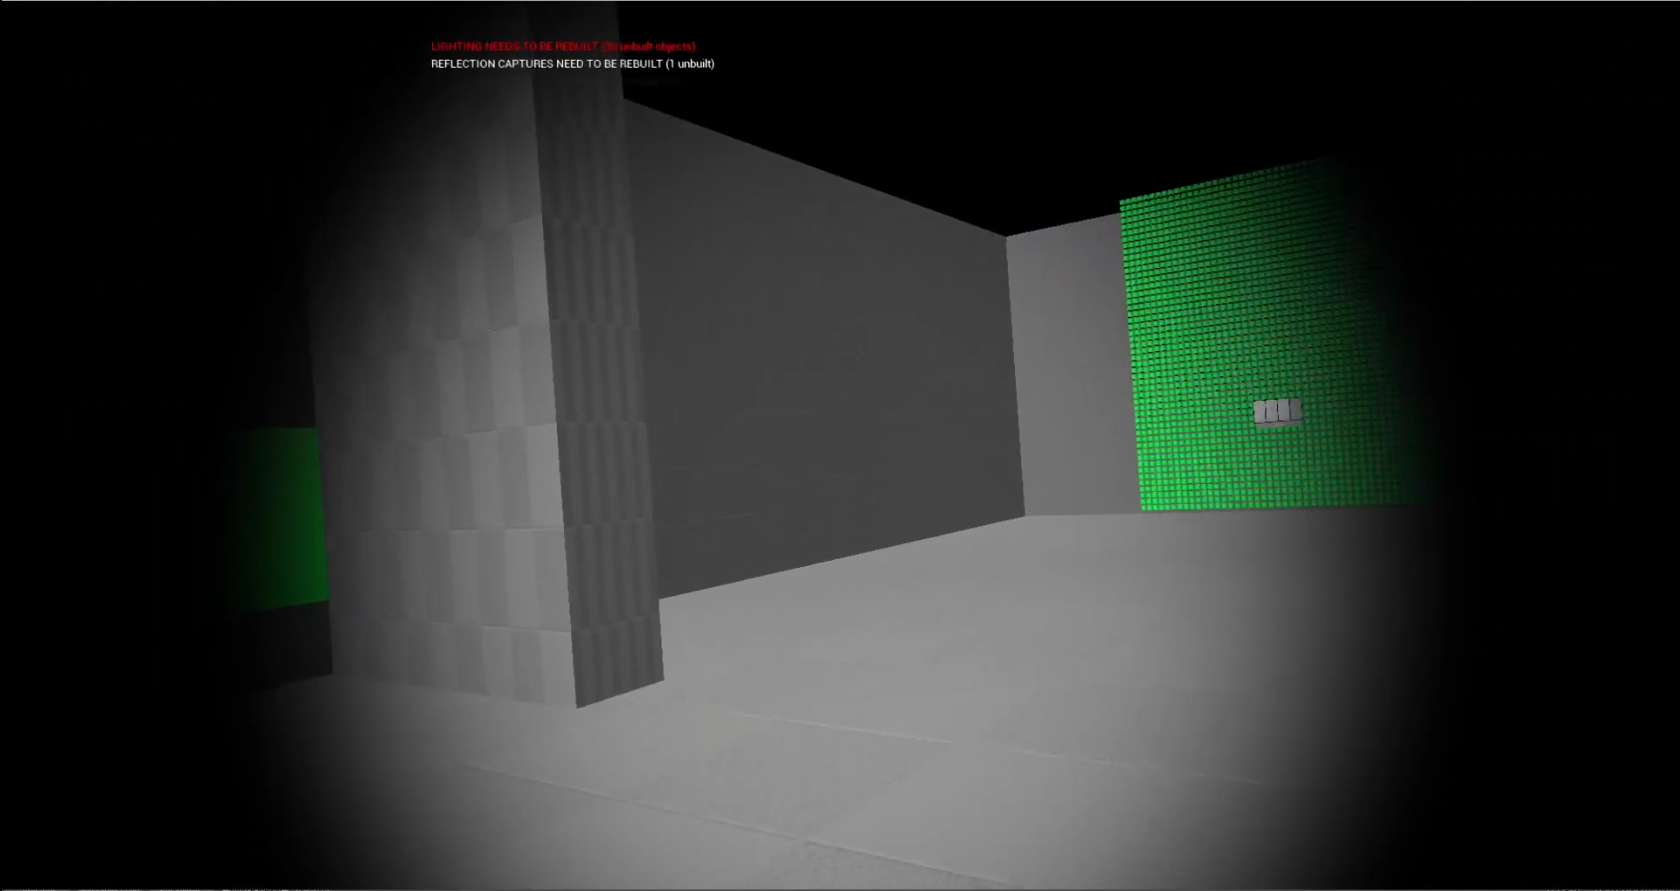
\includegraphics[width=0.8\linewidth]{graphics/tunnelvisionUE4.png}
		\caption{Wizja tunelowa}	
		\label{ref:subref_a}
	\end{subfigure}%

	\begin{subfigure}{.8\textwidth}
		\centering
		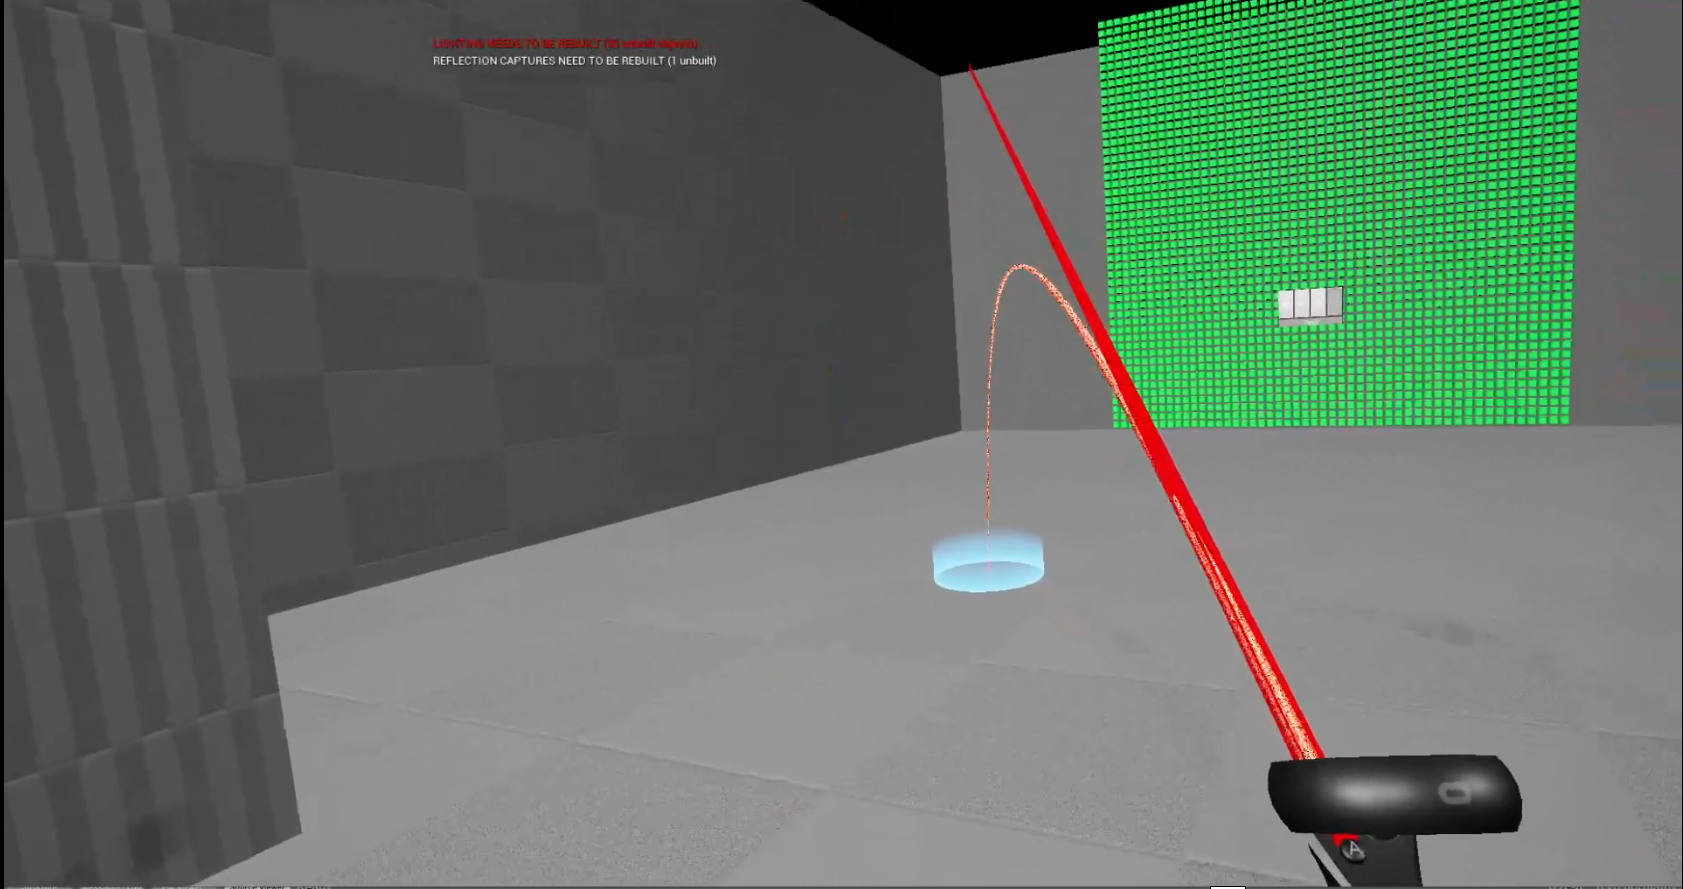
\includegraphics[width=0.8\linewidth]{graphics/teleportmoveUE4.png}
		\caption{Ruch teleportacyjny}	
		\label{ref:subref_c}
	\end{subfigure}%

\caption{Sposób poruszania się w programie.}
\label{ref:ref}
\end{figure}



\newpage
\subsection{Wygląd Galerii w Programie}

Każdy pokój został podzielony na dwie części. W części pierwszej znajdują się informacje o modelu, jaki się znajduję w pokoju. Swoim wyglądem przypomina to galerię obrazów, do których można podejść i poczytać ciekawostki o modelu. W drugiej części znajduje się model komputerowy. W zależności od modelu możemy z nim wchodzić w interakcje, aby zobaczyć jak model działa w ruchu.

\begin{figure}[!ht]%
\centering
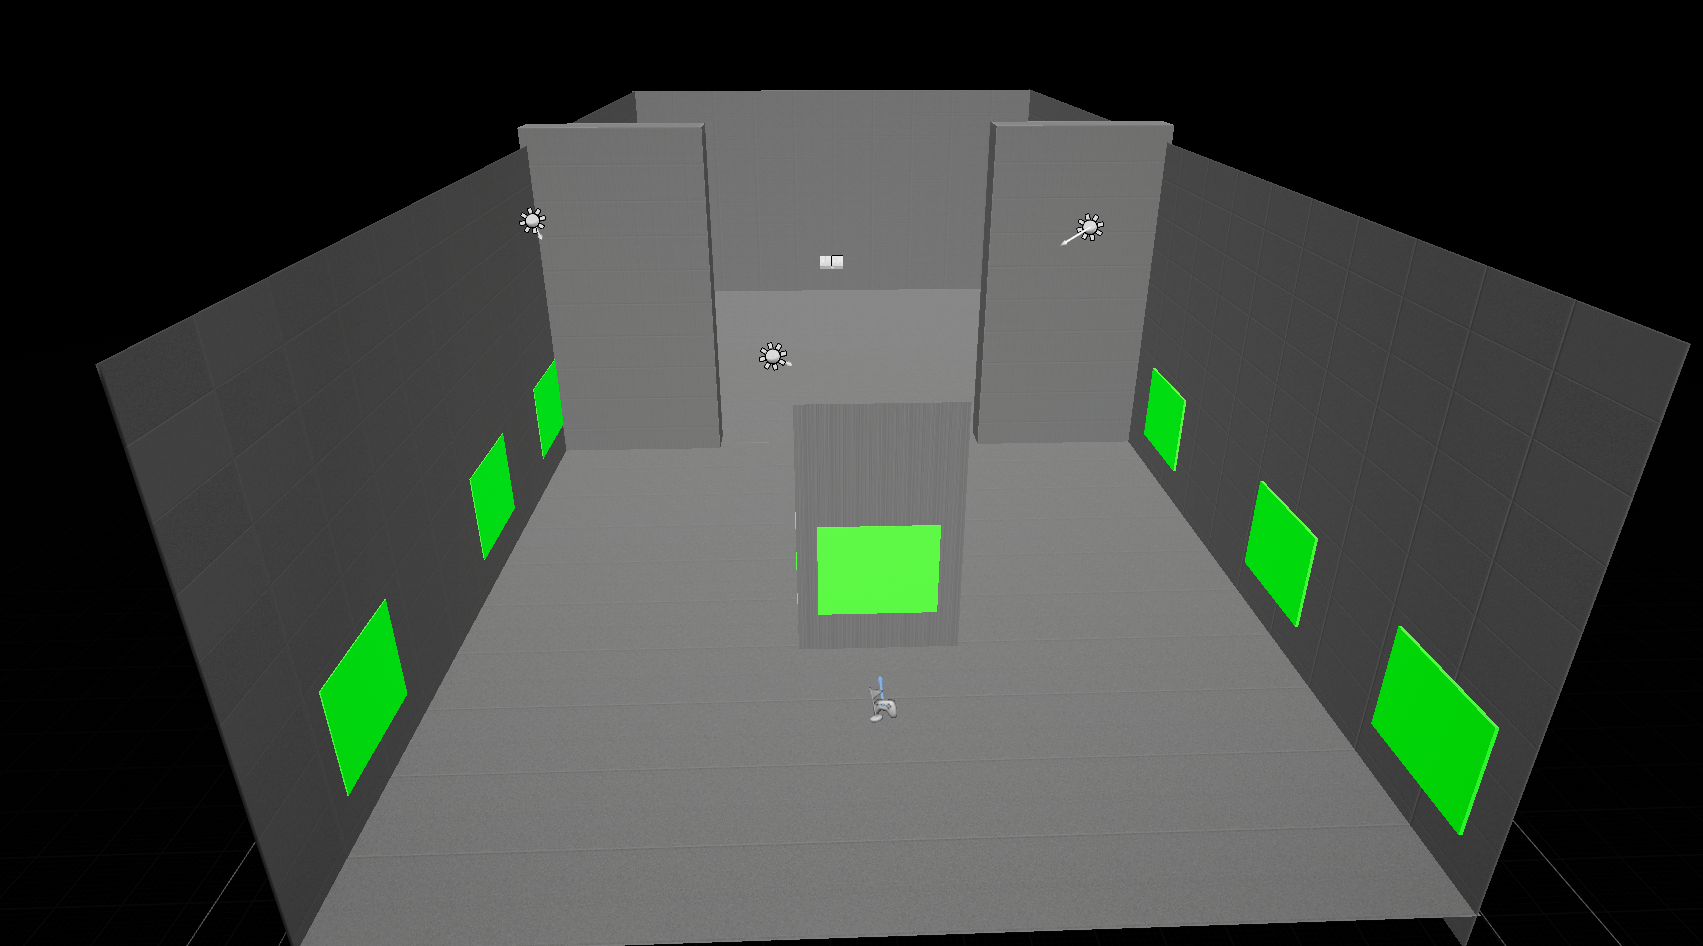
\includegraphics[width=0.8\columnwidth]{graphics/Level.png}
\caption{Wygląd pokoju galerii w programie.
\label{OpenBrush}}%
%
\qquad
\end{figure}  

\newpage
\section{Warstwa Programistyczna}

\subsection{Unreal Engine 4}

Program został napisany na silniku Unreal Engine 4. Został on wybrany z powodu wsparcia gogli VR, dużej społeczności, otwartego kodu źródłowego oraz możliwość pisania kody w języku C++. Dzięki wsparci gogli VR nie trzeba tracić czasu, by napisać odpowiednie narzędzie do ich obsługi. Duża społeczność oznacza, że w internecie można znaleźć wiele pomocnych materiałów przy tworzeniu aplikacji. Otwartość kodu oznacza, że można bez większych problemów wprowadzić własne modyfikacje, jeśli są potrzebne. Jedną z najważniejszych funkcji UE4 jest Unreal Editor, czyli graficzny edytor silnika, w którym bez znajomości programowania można stworzyć własny program. Kolejną ważną funkcja UE4 jest wbudowany język skryptowy zwany BluePrint. Jest on oparty na koncepcji wykorzystywania interfejsu opartego na węzłach, dzięki którym możemy tworzyć elementy programu bezpośrednio w Unreal Editor bez wchodzenia do kodu źródłowego C++. Jest on używany do definiowania klas lub obiektów metodą programowania obiektowego.

\begin{figure}[!ht]%
\centering
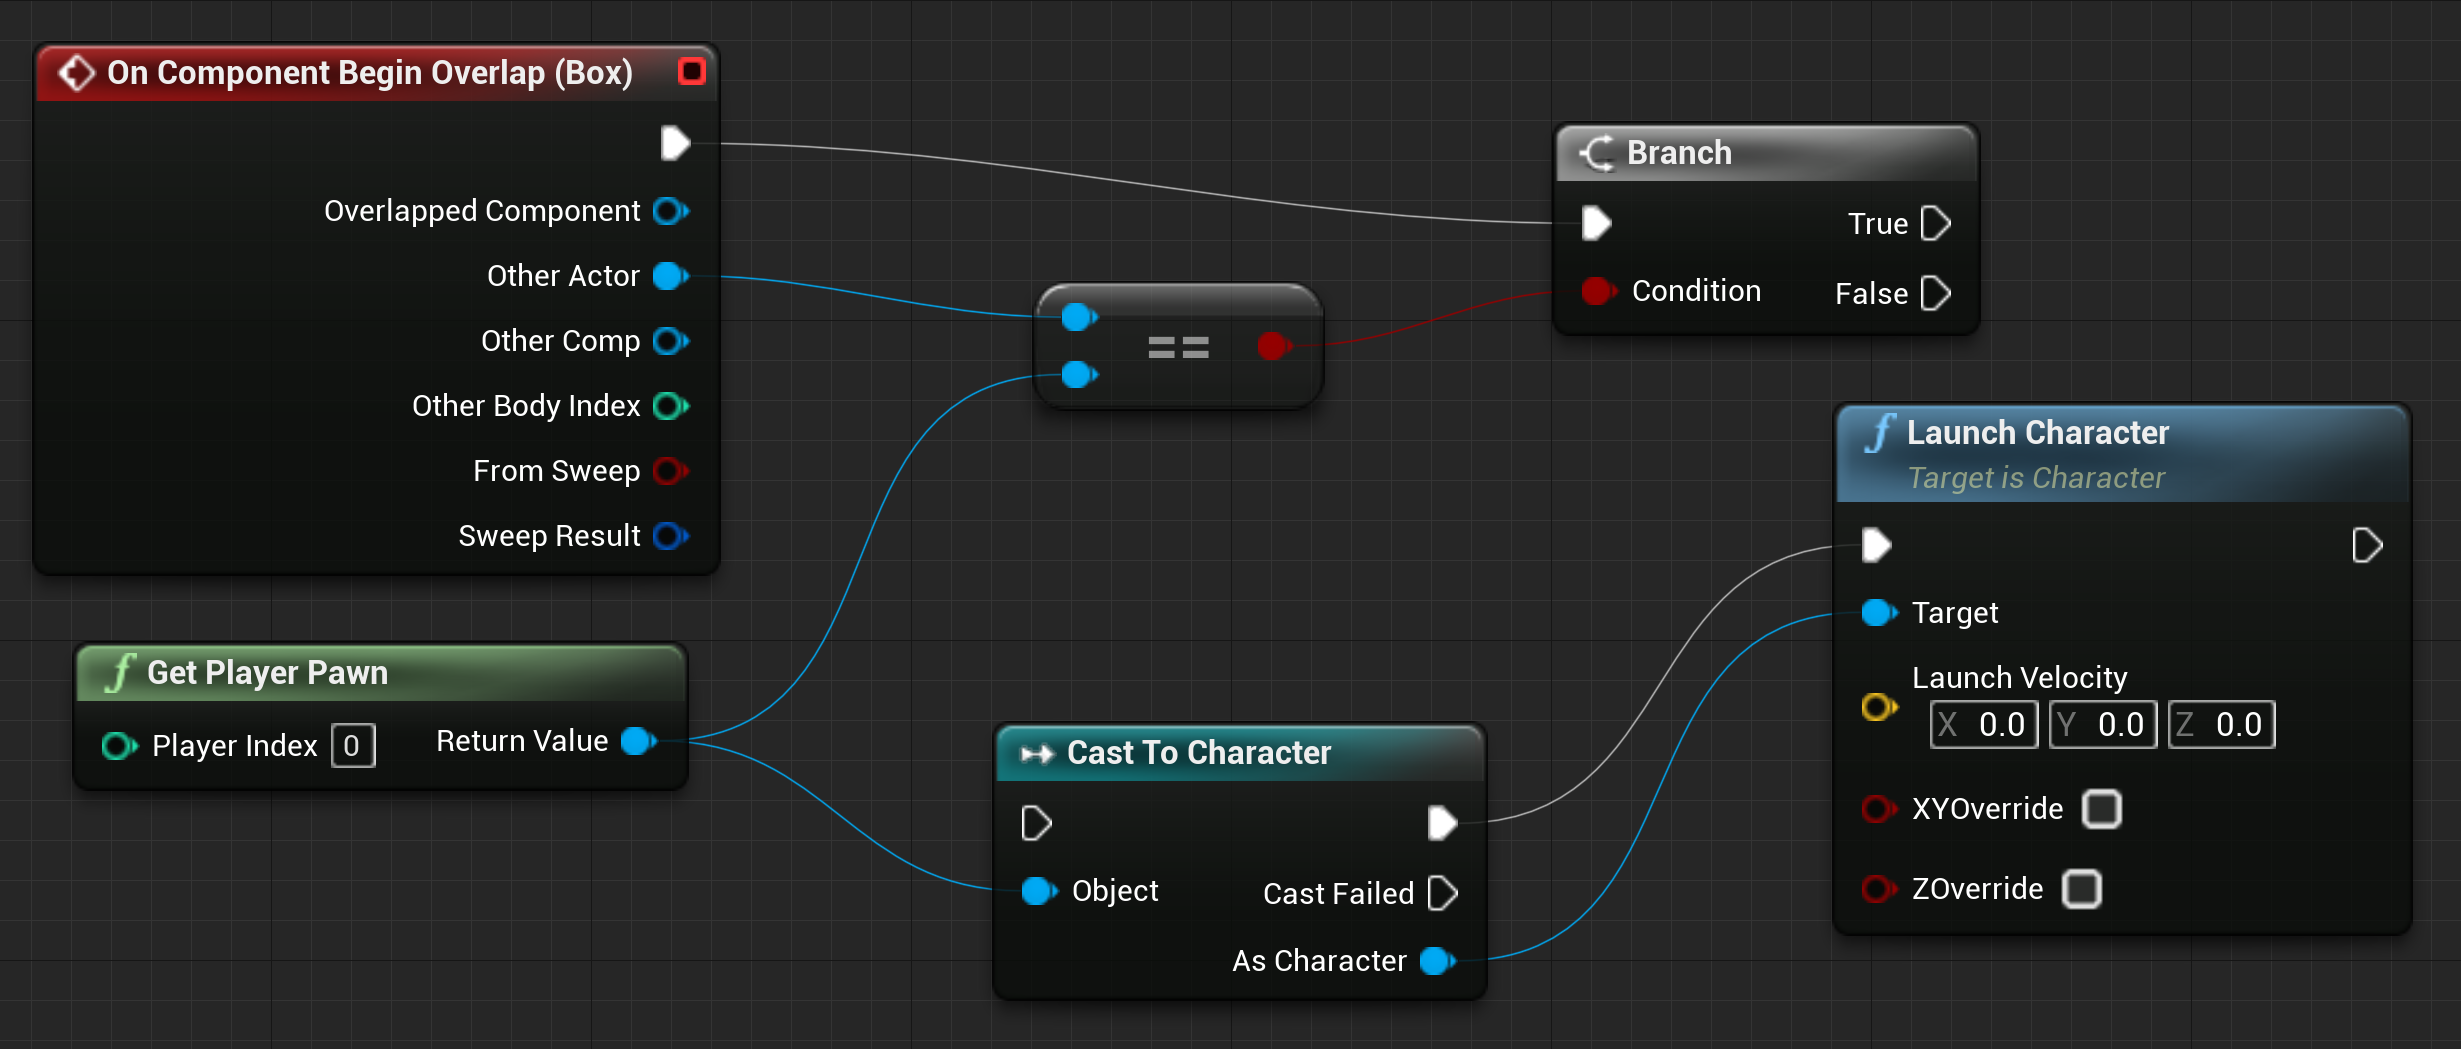
\includegraphics[width=1\columnwidth]{graphics/BPExample.png}
\caption{Przykładowa funkcja napisana w unrealowych blueprintach.
\label{BPExample}}%
%
\qquad
\end{figure}  

Unreal Editor pozwala też na tworzenie poziomów w prosty i intuicyjny sposób, poprzez przeciąganie interesującego nas obiektu bezpośrednio na ekran, a następnie zmiany jego obrotu czy skali. Edytor pozwala również na uruchomienie obecnie włączonego poziomu, by zobaczyć czy wszystkie funkcje zostały prawidłowo napisanie i nie ma żadnych z nimi problemów. Jeśli pojawi się jakiś problem BP pozwala na debugowanie funkcji, które zostały w nim napisane.
\subsection{Język C++}

Innym sposobem na tworzenie nowej funkcjonalności dla tworzonego programu w Unreal Engine jest napisanie jej w C++. Klasy C++ mogę być używane jako klasy bazowe dla klas BluePrintowych, gdzie podstawy klasy tworzymy w C++, a następnie rozszerzamy jej możliwość w BP. C++ pozwala na tworzenie metod i zmiennych, które następnie mogą być wykorzystane w BP, dzięki odpowiednim specyfikatorom. Dla metod używany jest UFUNCTION z odpowiednimi flagami w zależności od tego, jak dana metoda ma się zachować w BP. Dzięki temu można na przykład w BP odwołać się do metody stworzonej w C++ i korzystać z niej jakby była stworzona w BP. Ma to swoje zalety, z czego największą jest to, że metody w C++ są szybsze niż ich odpowiedniki w BP. Podobnie jak dla metod zmienne też posiadają swój specyfikator UPROPERTY, dzięki któremu zmienne stworzone w C++ możemy użyć w BP.


\lstinputlisting[caption=Przykład kodu C++, label={lst:listing-cpp}, language=C++]{code/03/BoidTarget.cpp}

\subsection{Oculus Quest}

Gogle VR, które były wykorzystywane do testowania projektu to Oculus Quest. Gogle posiadają dwa ekrany OLED o rozdzielczości 1440x1600 na każdy ekran. Częstotliwość odświeżania ekranów wynosi 72 Hz. Do obsługi gogli wykorzystywane są dwa kontrolery Oculus Touch drugiej generacji. Dzięki swojej autonomiczności nie potrzeba podłączać gogli bezpośrednio do komputera, lecz można wykorzystać lokalną sieć WiFi i oficjalne oprogramowanie firmy Reality Labs. Natomiast dzięki oficjalnemu wsparciu w Unreal Engine można od razu po stworzeniu nowego projektu, zacząć pisać go z myślą o goglach VR.


\section{Modele wykorzystane w programie}

\subsection{Wahadło Podwójne}

Pierwszy model, który został umieszczony w projekcie to model wahadła podwójnego. Wahadło podwójne składa się z dwóch wahadeł prostych, tzn. pierwsze wahadło o masie $m_0$ zostało przymocowane za pomocą pręta o długości $l_0$ do stałego punktu obrotu, gdzie $\theta_0$ jest przesunięciem kątowym wahadła od położenia równowagi. Drugie wahadło o masie $m_1$ zostało przymocowane za pomocą pręta o długości $l_1$ do pierwszego wahadła z własnym kątem swobody $\theta_1$. Z powodu występowania dwóch stopni swobody $\theta_0$ i $\theta_1$, a przez to ma bardziej złożony ruch, wahadło jest podatne na chaotyczny ruch i jest bardzo wrażliwy na warunki początkowe  \cite{double_pendulum_book}.

\begin{figure}[!ht]%
\centering
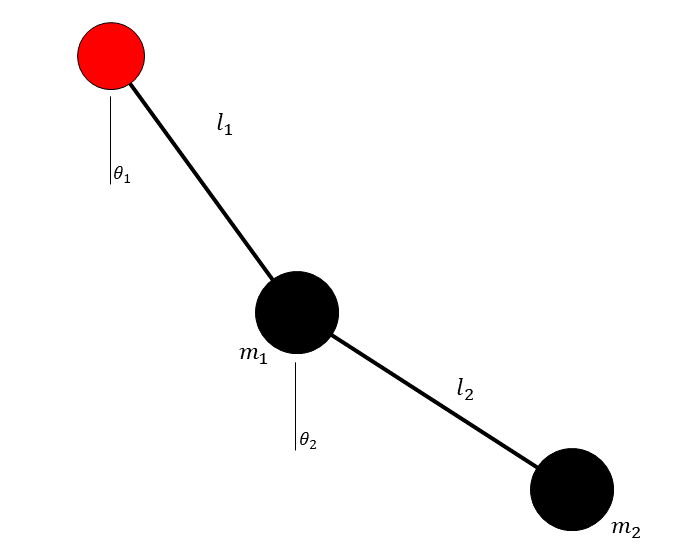
\includegraphics[width=0.5\columnwidth]{graphics/pendulum/DoublePendulum.png}
\caption{Wahadło podwójne.
\label{BPExample}}%
%
\qquad
\end{figure}  

\subsubsection{Wahadło podwójne - kod}


Aby obliczyć wartość $\theta_0$ i $\theta_1$ potrzebne są najpierw prędkości kątowe  $\dot{\theta_0}$ i $\dot{\theta_1}$ oraz ich przyśpieszenie kątowe $\ddot{\theta_0}$ i $\ddot{\theta_1}$. Aby obliczyć zmianie kąta w czasie trzeba rozwiązać układ równań różniczkowych. Najpierw robimy do dla kątów  $\theta_0$ i $\theta_1$, gdzie pochodna kąta od czasu jest równa $\dot{\theta_0}$ i $\dot{\theta_1}$. Zapisujemy równanie na pochodną prędkości od czasu dla $\dot{\theta_0}$ i $\dot{\theta_1}$ co daje nam przyśpieszenie kątowe $\ddot{\theta_0}$ i $\ddot{\theta_1}$.

\begin{equation}
\begin{split} 
\frac{\partial\theta_0}{\partial t}=\dot{\theta_0}
\\
\frac{\partial\theta_1}{\partial t}=\dot{\theta_1}
\\
\frac{\partial\dot{\theta_0}}{\partial t}=\ddot{\theta_0}
\\
\frac{\partial\dot{\theta_1}}{\partial t}=\ddot{\theta_1}
\end{split}
\label{thetas}
\end{equation}

Równania [\ref{thetas}] możemy zapisać jako równanie różnicowe, tzn. dokonujemy przekształcenia, w którym pochodną po czasie zastępujemy prostym operatorem liniowym:

\begin{equation}
\begin{split} 
\theta_0=\theta_0+\dot{\theta_0}*dt;
\\
\theta_1=\theta_1+\dot{\theta_1}*dt;
\\
\dot{\theta_0}=\dot{\theta_0}+\ddot{\theta_0}*dt;
\\
\dot{\theta_1}=\dot{\theta_1}+\ddot{\theta_1}*dt;
\\
gdzie:
\\
dt-krok\ czasowy
\end{split}
\label{pendumalgeb}
\end{equation}

Jest to realizacja metody Eulera. Brakuje nam już tylko $\ddot{\theta_0}$ i $\ddot{\theta_1}$, które można wyprowadzić ze wzoru \cite{double_pendulum}: 

\begin{equation}
\begin{split} 
\ddot{\theta_0}=\frac{g(\sin\theta_1\cos(\theta_0-\theta_1)-\mu\sin\theta_0)
-(l_1\dot{\theta_1^2}+l_0\dot{\theta_0^2}\cos(\theta_0-\theta_1))\sin(\theta_0-\theta_1)}{l_0(\mu-\cos^2(\theta_0-\theta_1))}
\\
\ddot{\theta_1}=\frac{g\mu(\sin\theta_0\cos(\theta_0-\theta_1)-\sin\theta_1)
-(\mu l_0\dot{\theta_0^2}+l_1\dot{\theta_1^2}\cos(\theta_0-\theta_1))\sin(\theta_0-\theta_1)}
{l_1(\mu-\cos^2(\theta_0-\theta_1))}
\\
gdzie:
\\
\mu=1+(m_0+m_1)
\end{split}
\label{computeAngularAcceleration}
\end{equation}

Kod C++ przeznaczony do tworzenia i zarządzania wahadłami składa się z trzech klas: Pendulum, PendulumSpawn, PendulumControl.

Tak wyżej utworzone równania możemy wykorzystać w kodzie do obliczenia wartości $\theta_0$ i $\theta_1$ w danym kroku czasowym.

\lstinputlisting[caption=Obliczanie wartości $\theta_0$ i $\theta_1$, label={lst:listing-cpp}, language=C++]{code/doublependulum/ComputeAnglesEuler.cpp}
\label{ComputeTheta}

%spytać się o ref do listingu

Tak wyliczone wartości $\theta_0$ i $\theta_1$ są wykorzystane do obliczenia położeń wahadeł w kolejnej funkcji. Pręta wahadeł są stworzone ze "Spline Mesh Compoment", jest to zdeformowany Static Mesh, w którym podajemy mu obecnie wyliczone współrzędne wahadła, dzięki temu uzyskujemy odpowiednio wyglądające wahadło.

\lstinputlisting[caption=Aktualizacja pozycji wahadła, label={lst:listing-cpp}, language=C++]{code/doublependulum/ComputePosition.cpp}


Klasa PendulumSpawn jest natomiast odpowiedzialna za dodawanie, usuwanie wahadeł. Klasa jest też odpowiedzialna za uruchomianie i resetowanie wszystkich wahadeł, które zostały przez dany PendulumSpawn stworzone.

Ostatnią klasą jest klasa PendulumControl, w której są zawarte metody i zmienne potrzebne do stworzenia interfejsu użytkownika, odpowiedzialnego za kontakt między użytkownikiem programu, a PendulumSpawn.

\subsubsection{Wahadło podwójne - UE4}

Na podstawie klas C++ z poprzedniego podrozdziału stworzone zostały klasy BP.


W klasie BP\_Pendulum w blueprincie do najważniejszej rzeczy, którą można zrobić, jest możliwość zmiany siatki 3D i materiału, z którego jest stworzone wahadło:

\begin{figure}[!ht]%
\centering
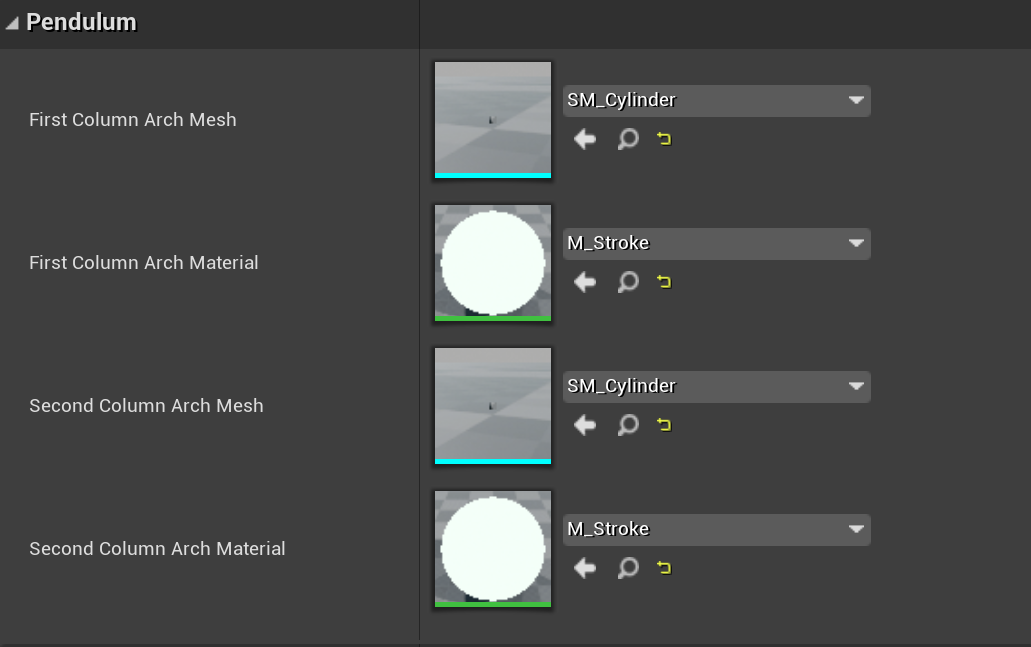
\includegraphics[width=0.7\columnwidth]{graphics/pendulum/PendulumBP.png}
\caption{Ustawiony mesh i tekstura dla wahadła .
\label{BPExample}}%
%
\qquad
\end{figure}  

W klasie BP\_PendulumSpawn ustawiamy tylko jakie ma tworzyć wahadła oraz jaki widget ma być umieszczony do obsługi wahadeł. Po ustawieniu wszystkich potrzebnych rzeczy klasę można umieścić na poziomie:

\begin{figure}[!ht]%
\centering
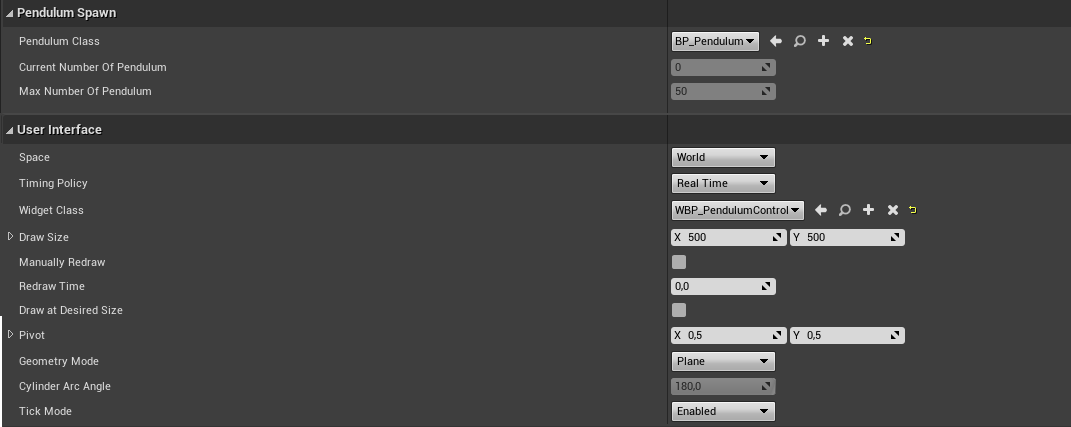
\includegraphics[width=0.7\columnwidth]{graphics/pendulum/PendulumSpawnerBP.png}
\caption{Ustawione wahadło do stworzenia i widget.
\label{BPExample}}%
%
\qquad
\end{figure}  

 
Klasa WBP\_PendulumControl jest klasą typu widget, czyli klasą interfejsu użytkownika. W klasie tej trzeba stworzyć odpowiednie jej elementy na podstawie bazowej klasy C++, aby móc obsługiwać wahadła stworzone przez BP\_PendulumSpawn


\begin{figure}[!ht]%
\centering
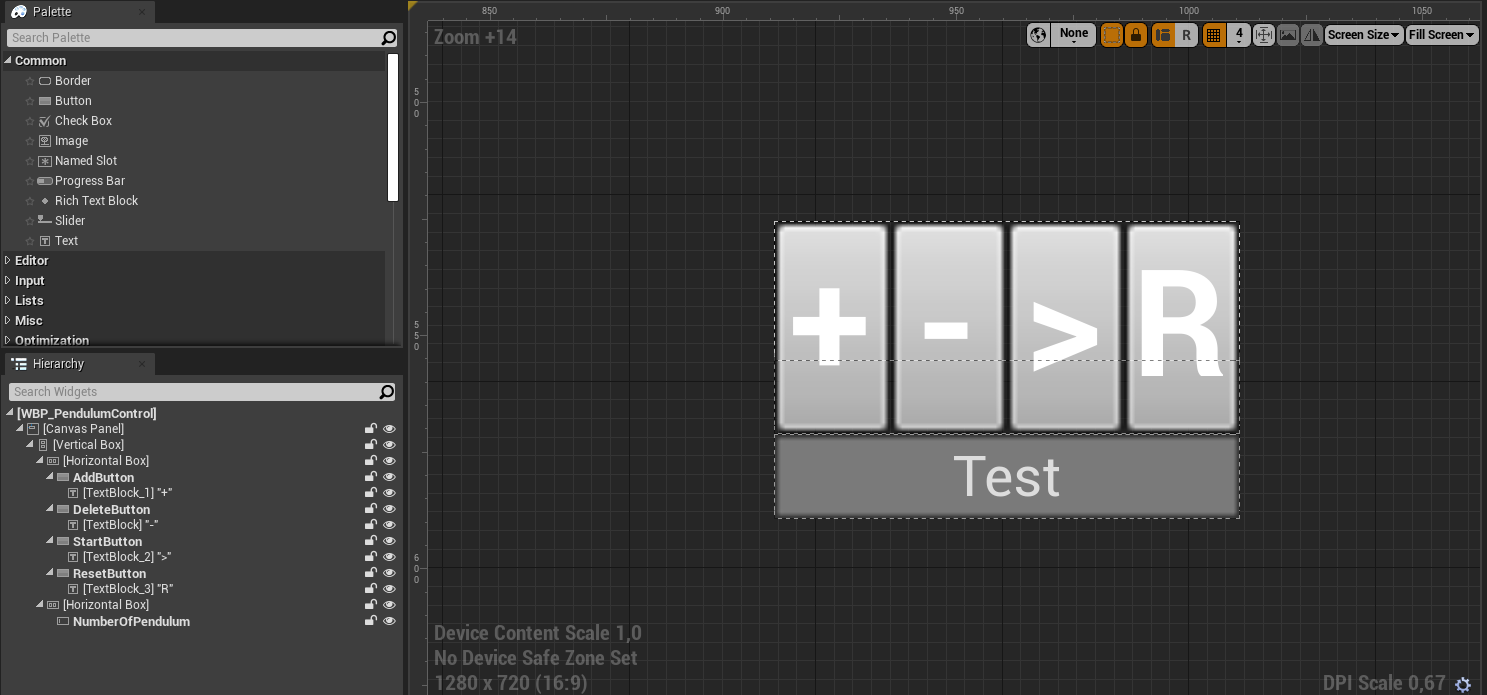
\includegraphics[width=0.7\columnwidth]{graphics/pendulum/PendulumControlBP.png}
\caption{Wygląd widgetu w programie.
\label{BPExample}}%
%
\qquad
\end{figure}  

\newpage
\subsubsection{Wahadło podwójne – Wygląd symulacji w projekcie}

W projekcie po najechaniu wskaźnikiem z kontrolera ruchowego na panel użytkownika możemy dodać, usunąć, uruchomić lub zresetować wahadła stworzone przez spawner. Jak pokazano na rysunku \ref{Pendulum_in_project:subref_a}, na początku symulacji wahadła są stosunkowo blisko siebie. Lecz w trakcie jej działania w pewnym momencie wahadła zaczną się zachowywać w sposób chaotyczny, tak jak to widać na rysunku \ref{Pendulum_in_project:subref_b}.


\begin{figure}[!ht]%
	\centering
	\begin{subfigure}{.5\textwidth}
		\centering
		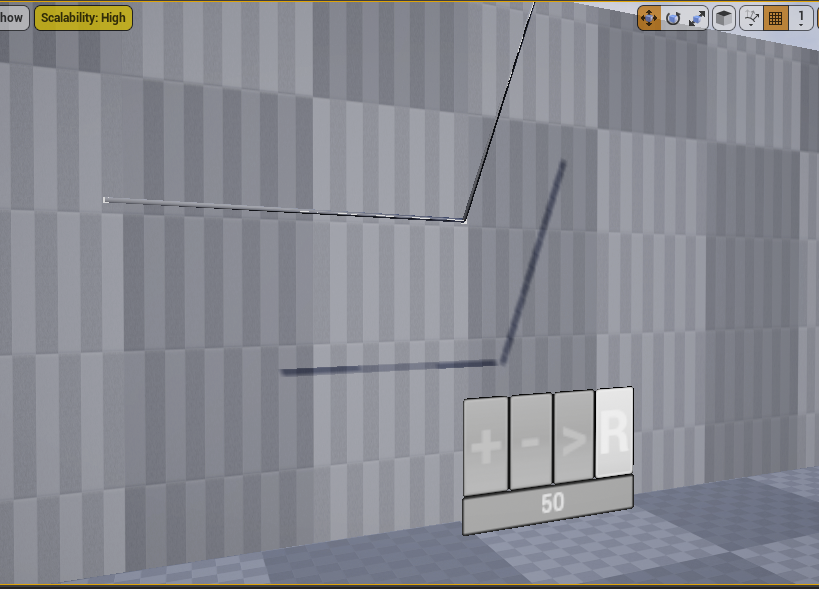
\includegraphics[width=.95\linewidth]{graphics/pendulum/PendulumInUE_1.png}
		\caption{Wahadła na początku symulacji.}	
		\label{Pendulum_in_project:subref_a}
	\end{subfigure}%
	\hfill
	\begin{subfigure}{.5\textwidth}
		\centering
		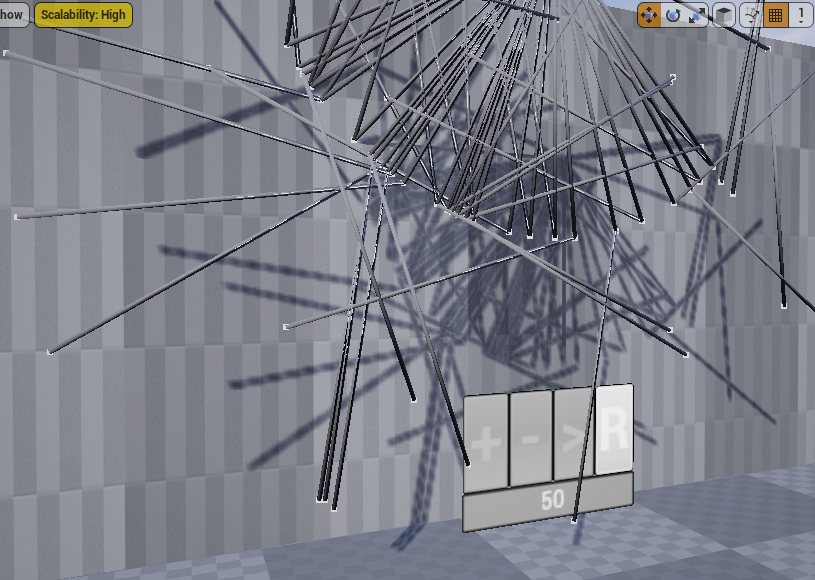
\includegraphics[width=.95\linewidth]{graphics/pendulum/PendulumInUE_2.png}
		\caption{Wahadła na końcu symulacji.}
		\label{Pendulum_in_project:subref_b}
	\end{subfigure}%
	

\caption{Działanie postępowania symulacji wahadeł.}
\label{Pendulum_in_project}
\end{figure}

\newpage
\subsection{Gra w życie}

Gra w życie, jest automatem komórkowym stworzonym przez Johna Conwaya. Jest to sieć komórek, symulowanych w pamięci komputera, w którym w danej chwili każda z komórek przyjmuje określony stan, według wcześniej ustanowionych reguł \cite{game_of_life_zero_cellular_automata}. 

John Conway zainteresował się problemem przedstawionym w latach 40 XX wieku przez matematyka Johna von Neumanna, który to próbował znaleźć hipotetyczną maszynę, która mogłaby budować kopie samej siebie. Neumannowi udało się, gdy znalazł matematyczny model takiej maszyny z bardzo skomplikowanymi regułami na prostokątnej siatce. Gra w życie powstała jako udana próba Conwaya uproszczenia idei von Neumanna \cite{game_of_life_story}. Gra w życie Conwaya pierwotnie ukazała się w październiku 1970 roku w magazynie "Scientific American" w kolumnie "Mathematical Games" Martina Gardnera, pod tytułem: "The fantastic combinations of John Conway's new solitaire game 'life'" \cite{game_of_life_methematical_games}, gdzie z miejsca zdobyła ogromną popularność.


 Sama Gra w życie nie jest do końca grą. Conway nazywał ją "gra bez graczy", czyli gra w której przebieg jest niezależny od gracza, a jego rola sprowadza się w tym wypadku tylko do utworzenia stanu początkowego, czyli pierwszej generacji komórek \cite{game_of_life_zero_player}. 


 Gra w pierwotnym założeniu rozgrywa się na 2 wymiarowej siatce składającej się z komórek. Każda komórka w danej turze (generacji) może być albo żywa, albo martwa. To czy pojedyncza komórka w kolejnej turze będzie żyć lub nie, zależy od stanu jej 8 sąsiadów i ustanowionych początkowych reguł.

\begin{figure}[!ht]%
\centering
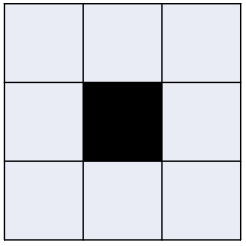
\includegraphics[width=0.2\columnwidth]{graphics//gameoflife/GOL_Cell.png}
\caption{Pojedyncza komórka i 8 sąsiadów w grze w życie.
\label{BPExample}}%
%
\qquad
\end{figure} 

Gra w życie w pierwotnych założeniach składa się z 4 zasad \cite{game_of_life_story}:

\begin{itemize}
\item Każda żywa komórka z mniej niż dwoma żywymi sąsiadami umiera
\item Każda żywa komórka mająca więcej niż trzech żywych sąsiadów umiera
\item Każda żywa komórka z dwoma lub trzema żywymi sąsiadami żyje, niezmieniona, do następnego pokolenia.
\item Każda martwa komórka z dokładnie trzema żywymi sąsiadami ożywa.
\end{itemize}


Na podstawie kodu \cite{game_of_life_code} została stworzona wersja Gry w Życie, która działa z kontrolerami ruchów VR.
\subsubsection{Gra w życie - kod}

W C++ kod gry w życie składa się z trzech klas: CellActor, GridActor, GameOfLifeControl

CellActor jest klasą, w której znajdują się informację o jednej komórce znajdującej w siatce. W klasie znajdują się informację o położeniu na dwuwymiarowej siatce (X i Y), również informację o stanie życia w obecnej generacji oraz o stanu życia w kolejnej generacji. Klasa posiada metodę Clicked, dzięki której jak użytkownik wejdzie w interakcje z komórką zmienia jej status początkowy z martwej na żywą i vice versa. 

\lstinputlisting[caption=Aktualizacja stanu danej komórki przez użytkownika, label={lst:listing-cpp}, language=C++]{code/gameoflife/CellActorClicked.cpp}

Metoda Update, która jest wykorzystywana przez GridActora, podobnie jak metoda Clicked zmienia stan życia komórki, lecz w tym wypadku wykorzystuję zmienną AliveNext.

\lstinputlisting[caption=Aktualizacja stanu danej komórki, label={lst:listing-cpp}, language=C++]{code/gameoflife/CellActorUpdate.cpp}


Klasa GridActor jest odpowiedzialna za tworzenie dwuwymiarowej siatki składającej się z CellActorów i o podanej wysokości oraz długości. W klasie odbywają się wszystkie obliczenia związane z działaniem gry w życie od obliczania obecnie żyjących sąsiadów danej komórki w metodzie CountAliveNeighbors(const int i, const int j)

\lstinputlisting[caption=Zliczanie żyjących sąsiadów danej komórki, label={lst:listing-cpp}, language=C++]{code/gameoflife/GridActorCount.cpp}

Następnie na podstawie obecnie żyjących sąsiadów i reguł jakie zostały ustawione w metodzie UpdateAliveNext(const int Index, const int NumAliveNeighbors) ustawiamy czy dana komórka w następnej klatce będzie żywa lub martwa.

\lstinputlisting[caption=Aktualizacja stanu komórki w następnej klatce, label={lst:listing-cpp}, language=C++]{code/gameoflife/GridActorAlive.cpp}

Ostatnią klasą jest GameOfLifeControll która jest odpowiedzialna
za stworzenia interfejsu użytkownika, dzięki któremu użytkownik może włączyć grę w życie, zmieniać szybkość działania gry oraz resetować ją do stanu początkowego.
\subsubsection{Gra w życie - UE4}

Na podstawie powyższych klas zostały stworzone klasy BluePrintowe, które można potem umieścić w na poziomie w programie. W BP\_CellActor ustawiamy jak dana komórka ma wyglądać w świecie gry i jak się zachować, kiedy najedziemy na nią kontrolerem ruchowym:

\begin{figure}[!ht]%
	\centering
	\begin{subfigure}{.7\textwidth}
		\centering
		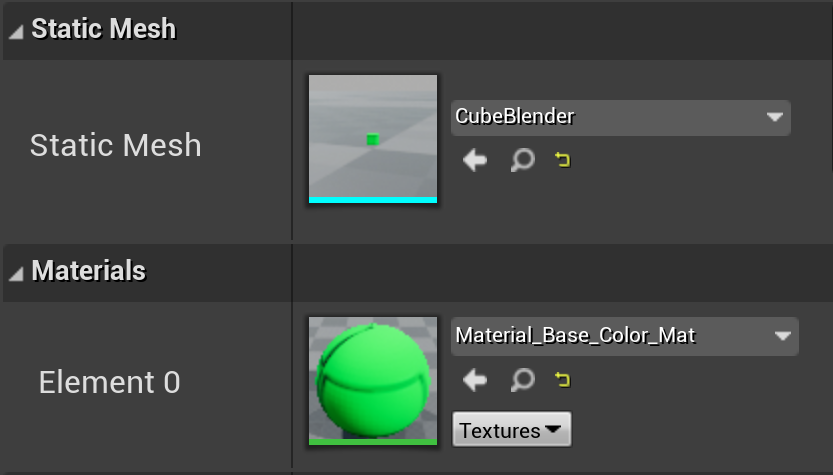
\includegraphics[width=0.8\linewidth]{graphics/gameoflife/CellActorInUE_1.png}
		\caption{Ustawiony mesh w programie dla komórki.}	
		\label{ref:subref_a}
	\end{subfigure}%
	
	\begin{subfigure}{.7\textwidth}
		\centering
		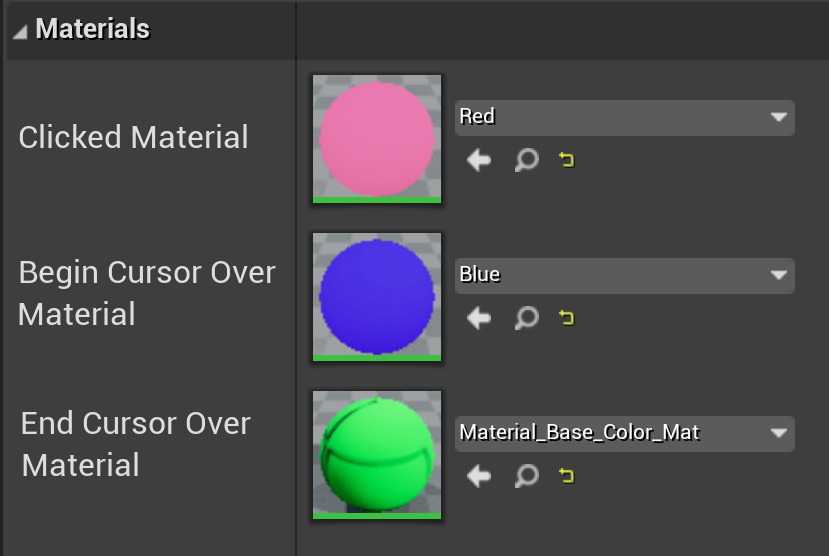
\includegraphics[width=0.8\linewidth]{graphics/gameoflife/CellActorInUE_2.png}
		\caption{Ustawiony wygląd w programie podczas akcji.}
		\label{ref:subref_b}
	\end{subfigure}%
	

\caption{Ustawienia dla CellActora w silniku Unreal.}
\label{ref:ref}
\end{figure}

BP\_GridActor2D jest klasą BluePrint, która znajdzie się na poziomie gry. W klasie ustawiamy, na jaką szerokość i wysokość ma zostać stworzona siatka składająca się z BP\_CellActor oraz dodajemy widget, dzięki któremu możemy sterować symulacją:

\begin{figure}[!ht]%
\centering
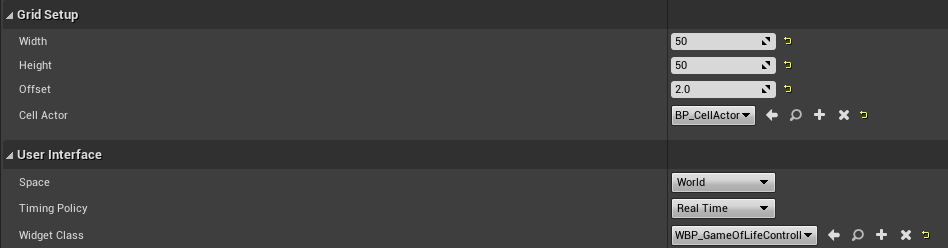
\includegraphics[width=0.6\columnwidth]{graphics/gameoflife/GridActor2DInUE_1.png}
\caption{Ustawienia BP\_GridActor2D.
\label{BPExample}}%
%
\qquad
\end{figure}  


Klasa WBP\_GameOfLifeControll jest odpowiedzialna kontakt między użytkownikiem a programem, klasa ta jest widgetem, dzięki któremu poprzez najechanie kontrolerem ruchowym na odpowiednie opcje możemy włączyć symulację, przyśpieszyć lub ją spowolnić oraz zresetować do stanu początkowego:

\begin{figure}[!ht]%
\centering
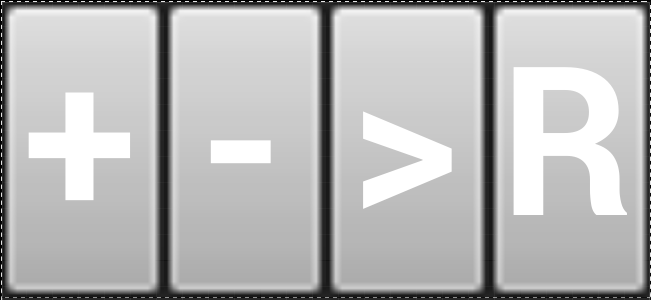
\includegraphics[width=0.7\columnwidth]{graphics/gameoflife/GameOfLifeControllInUE_1.png}
\caption{Wygląd widgetu w programie.
\label{BPExample}}%
%
\qquad
\end{figure}  

\subsubsection{Gra w życie - Wygląd symulacji w projekcie}
W programie za pomocą kontrolerów możemy ustawić stan początkowy każdej komórki w poprzez najechanie na nią wskaźnikiem wystającym z kontrolerów.

\begin{figure}[!ht]%
	\centering
	\begin{subfigure}{.5\textwidth}
		\centering
		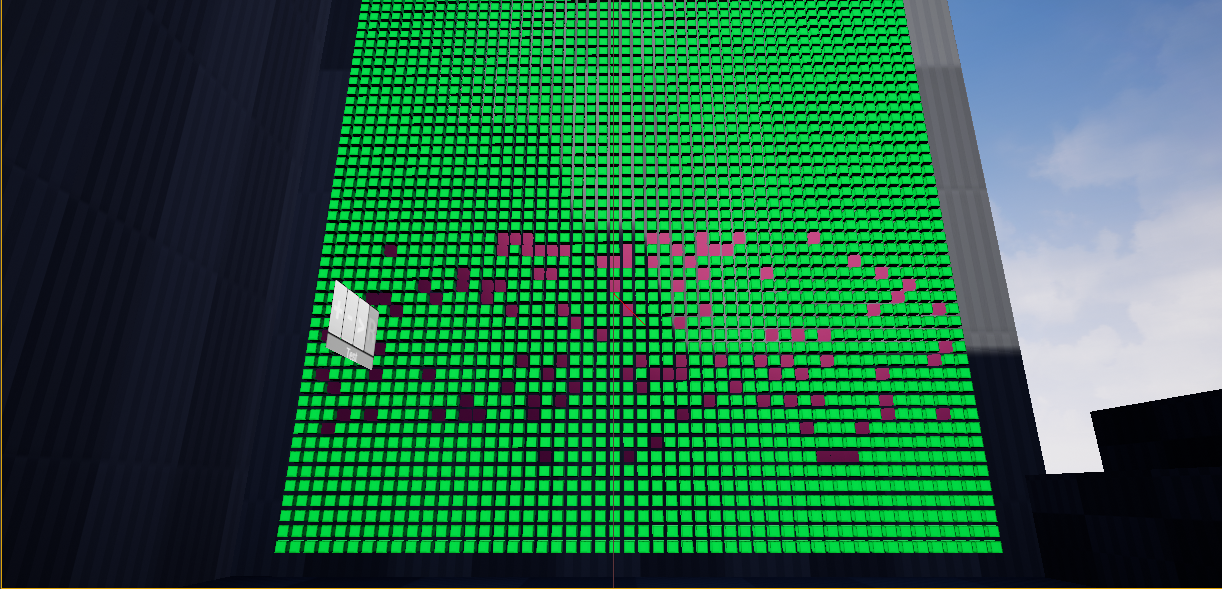
\includegraphics[width=0.9\linewidth]{graphics/gameoflife/GOLInUE_1.png}
		\caption{Ożywianie komórek z pomocą kontrolera}	
		\label{ref:subref_a}
	\end{subfigure}%
	\begin{subfigure}{.5\textwidth}
		\centering
		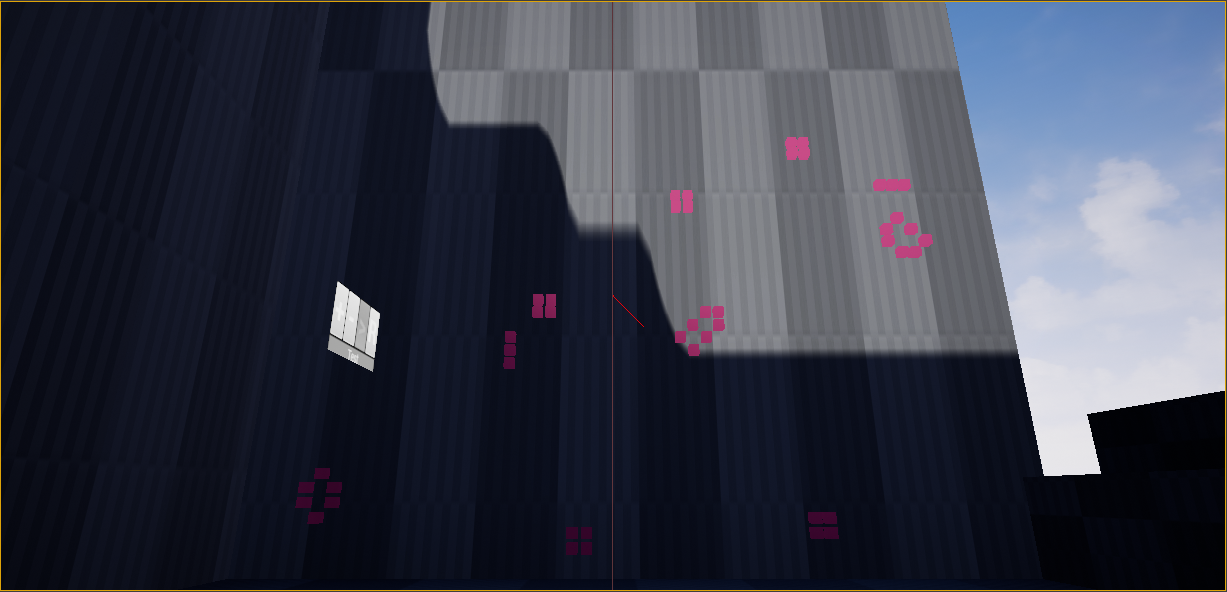
\includegraphics[width=0.9\linewidth]{graphics/gameoflife/GOLInUE_2.png}
		\caption{Uśmiercanie komórek z pomocą kontrolera}
		\label{ref:subref_b}
	\end{subfigure}%
\label{ref:ref}
\end{figure}

Po lewej stronie od tablicy z komórkami znajduje się widżet, za pomocą którego możemy włączyć grę, przyśpieszyć jej działanie lub spowolnić, albo zresetować komórki do stanu początkowego. 

\begin{figure}[!ht]%
	\centering
	\begin{subfigure}{.5\textwidth}
		\centering
		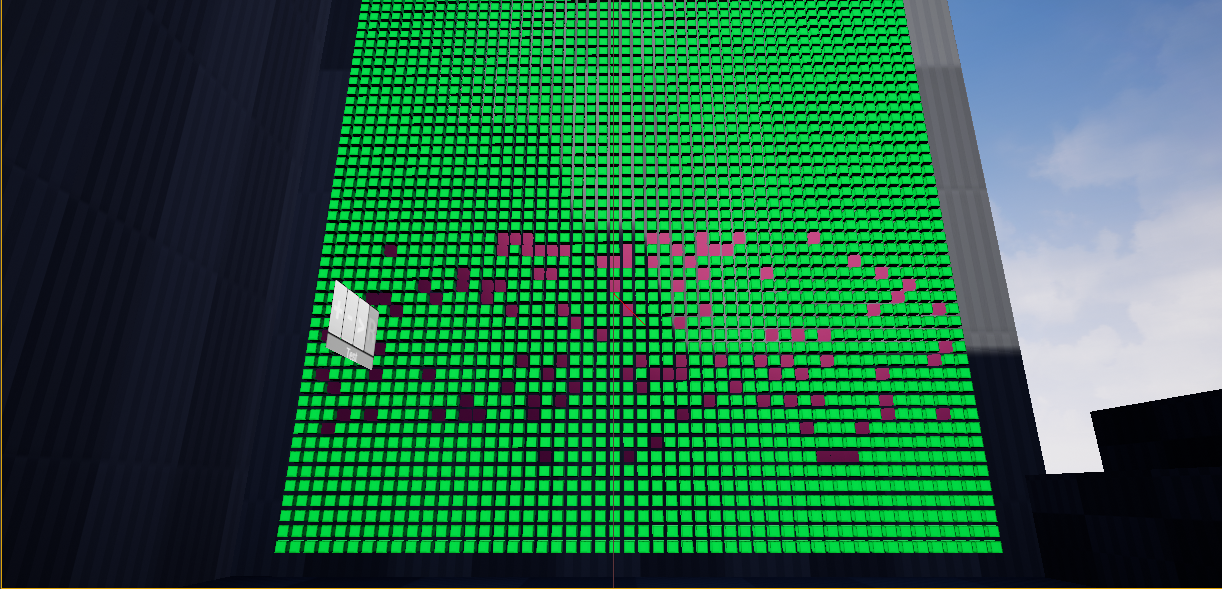
\includegraphics[width=0.9\linewidth]{graphics/gameoflife/GOLInUE_1.png}
		\caption{Wygląd tablicy z komórkami i widżetu}	
		\label{ref:subref_a}
	\end{subfigure}%
	\begin{subfigure}{.5\textwidth}
		\centering
		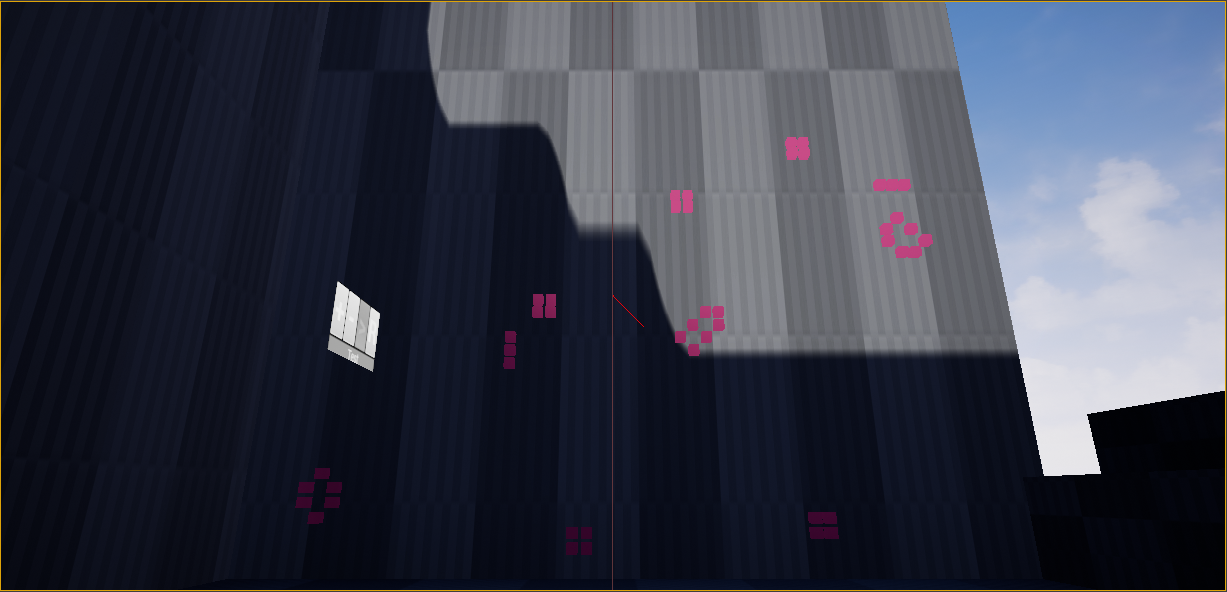
\includegraphics[width=0.9\linewidth]{graphics/gameoflife/GOLInUE_2.png}
		\caption{Wygląd tablicy w trakcie uruchomienia gry}
		\label{ref:subref_b}
	\end{subfigure}%
\label{ref:ref}
\end{figure}

\newpage
\subsection{Efekt Motyla}

"Czy trzepot skrzydeł motyla w Brazylii może wywołać tornado w Teksasie?" Jest to pytanie Edwarda Lorenza, meteorologa, który zadał je na 139 spotkaniu American Association for the Advancement of Science w stolicy USA w 1972 roku \cite{lorenz_praca}.
Lorenz jako pierwszy odkrył, że nie można zrobić dobrej prognozy pogody na dłużej niż kilka dni do przodu. W 1960 roku pracował on nad programem komputerowym, który miał prognozować pogodę, na podstawie zbioru równań określających zależności między prędkością wiatru, temperaturą, ciśnieniem i wilgotnością \cite{burze_motyle}. Gdy Lorenz testował swój program po wprowadzeniu danych i po wydrukowaniu wyniku w formie wykresu. Rozkład maksimów i minimów na wykresie wyglądał tak, jak się tego spodziewał Edward. Postanowił jednak ponownie zbadać wyniki, dlatego uruchomił program ponownie, wprowadzając jak myślał takie same wyniki \cite{burze_motyle}. Okazało się jednak, że wyniki wyszły na odwrót. Po sprawdzeniu danych zauważył, że podał je w postaci przybliżonej z mniejszą liczbą cyfr po przecinku. Było to dla niego tak ciekawe, że spróbował to samo z innymi zbiorami danych i zaobserwował identyczne zjawisko. Lorenz w ten sposób odkrył "efekt motyla", gdzie dla pewnych układów deterministycznych nawet minimalne zmiany wartości danych początkowych zostają bardzo szybko wzmocnione i powodują ogromne zmiany w ewolucji układu \cite{burze_motyle}.

\begin{figure}[H]%
\centering
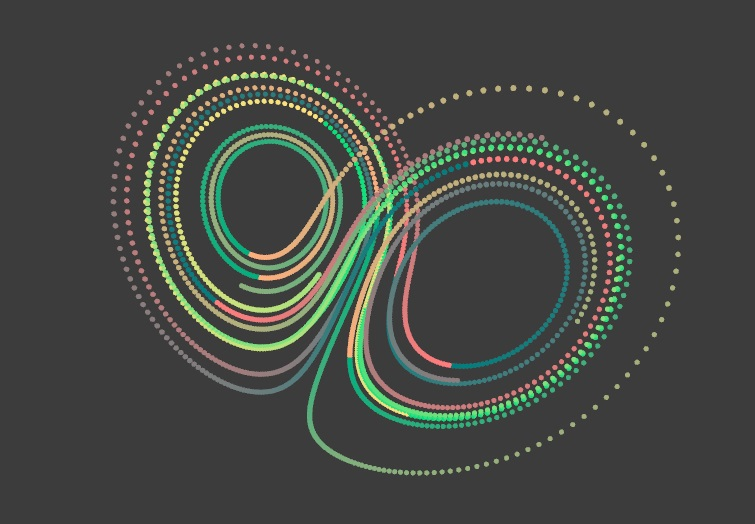
\includegraphics[width=0.7\columnwidth]{graphics/butterfly/Lorenz_Attractor.jpg}
\caption{Atraktor Lorenza 
\label{BPExample}}%
%
\qquad
\end{figure} 

Obecnie układ Lorenza jest bardziej znany jako układ 3 nieliniowych
równań różniczkowych \cite{lorenz_dziwne_atraktory}:

\begin{equation}
\begin{split}
\dot{x}=\sigma(y-x),\\
\dot{y}=x(\rho-z)-y,\\
\dot{z}=xy-\beta z,\\
\end{split}
\end{equation}
gdzie:\\
$\sigma$ - liczba Prandtla,\\
$\rho$ - liczba Rayleigha,\\
$\beta$ - obszar obejmujący równania\\
$\sigma$, $\rho$, $\beta$ > 0,\\
Jednakże zwykle podaje się \cite{lorenz_dziwne_atraktory}:\\
\begin{equation}
\begin{split}
\sigma = 10\\
\rho = 28\\
\beta - \frac{8}{3}
\end{split}
\label{ButterflyVariables}
\end{equation}

\subsubsection{Efekt Motyla - kod}

Kod C++ składa się z dwóch klas ButterflyActor i ButterflySpawner.
W ButterflyActor najważniejszą metodą jest Tick(float DeltaTime), w której poprzez rozwiązanie wcześniej pokazanych równań różniczkowych po przecałkowaniu. Następnie odpowiednio ustawiamy te równania dla pozycji X, Y i Z danego aktora \cite{motyle_cpp}

\lstinputlisting[caption=Metoda Tick(), label={lst:listing-cpp}, language=C++]{code/butterfly/ButterflyActorTick.cpp}

Jedyną rolą ButterflySpawner jest utworzenie tyle ButterflyActor ile zostanie mu zadane na początku, z drobną zmianą odległości dla każdego kolejnego aktora.


\lstinputlisting[caption=Tworzenie nowych atraktorów, label={lst:listing-cpp}, language=C++]{code/butterfly/ButterflySpawner.cpp}

\subsubsection{Efekt Motyla - UE4}

Na podstawie powyższych klas zostały stworzone klasy BluePrintowe, które można potem umieścić w na poziomie w programie. Dodatkowo dla BP\_ButterflyActor został stworzony efekt cząsteczkowy, który zostawia ścieżką jaką poruszał się dany aktor.
\begin{figure}[H]%
\centering
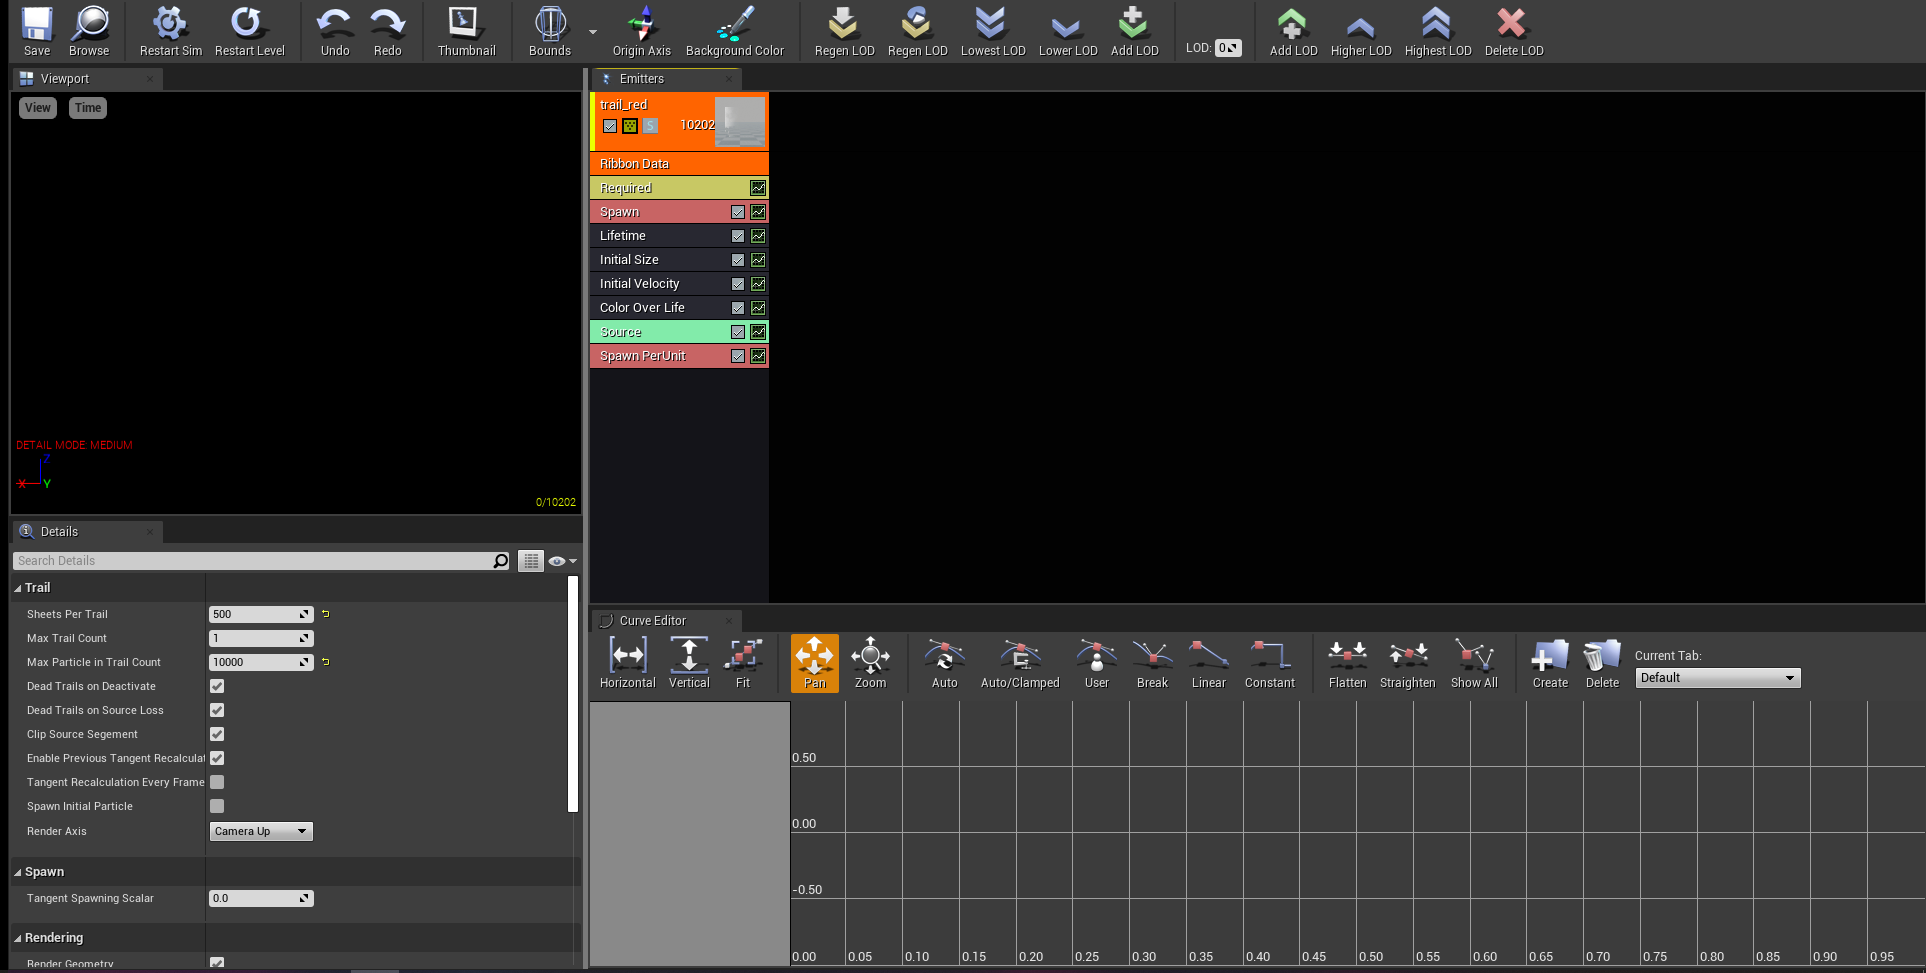
\includegraphics[width=0.9\columnwidth]{graphics/butterfly/ButterflyParticleSystem.png}
\caption{Wygląd menu do tworzenia efektów cząsteczkowych w UE4. 
\label{BPExample}}%
%
\qquad
\end{figure} 


W BP\_ButterflySpawner, w której ustawiamy ilość tworzonych atraktorów ich deltatime oraz sigma, rho i beta, które są wspólne dla wszystkich stworzonych atraktorów przez BP\_ButterflySpawner

\begin{figure}[H]%
\centering
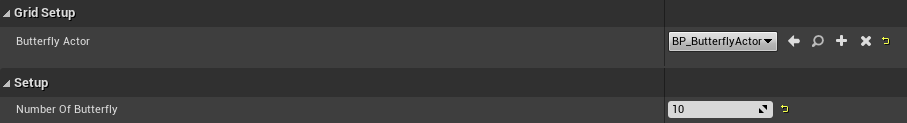
\includegraphics[width=0.7\columnwidth]{graphics/butterfly/ButterflySpawner.png}
\caption{Ustawienia BP\_ButterflySpawner.
\label{BPExample}}%
%
\qquad
\end{figure} 
\newpage
\subsubsection{Efekt Motyla - Wygląd symulacji w projekcie}

W programie użytkownik może obserwować układ Lorenza z wybranymi parametrami dla atraktorów [\ref{ButterflyVariables}], łącznie ze ścieżka, po jakiej się poruszają się atraktory. Dzięki temu może zobaczyć jak zmienia się zachowanie układu po zmienieniu wartości zmiennych

\begin{figure}[H]%
\centering
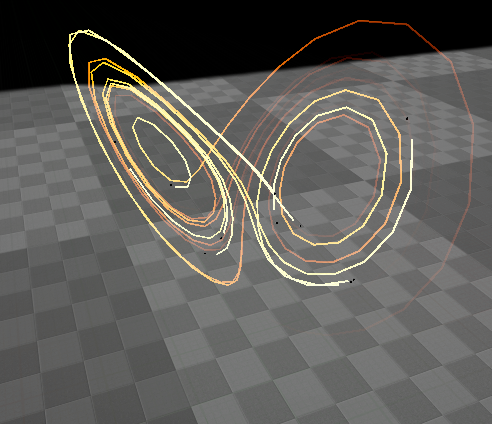
\includegraphics[width=0.9\columnwidth]{graphics/butterfly/ButterflyInUE_1.png}
\caption{Wygląd motyli w programie.
\label{ButterflyEffectUE4}}%
%
\qquad
\end{figure}  

\newpage
\subsection{Modele Agentowe}

Model agentowy jest typem modelu gdzie analizujemy wpływ agenta na dane środowisko i vice versa. Agentem może być np. komórka, człowiek, zwierzę itd. W modelu agentowym ustawiamy zachowanie poszczególnego lub grup agentów i obserwujemy jak wpływają na resztę w danym środowisku testowym. Główną ideą jest sprawdzenie, w jaki sposób czynniki w mikro skali wpływają na czynniki w środowisku makro. Dzięki temu możemy wykorzystać tak zdobytą wiedzę do różnych celów np. Sprawdzenie roznoszenia się epidemii, badać zachowania konsumenckie u ludzi czy tworzyć proste środowiska, by zobaczyć jak populacja danych agentów zmieniała się w czasie \cite{agent_examples}.

W projekcie został stworzony prosty model środowiska, gdzie są 3 rodzaje agentów: Rośliny, Króliki i Lisy. Celem królików jest rozmnożenie się poprzez znalezienie najbliższego królika do tego zdolnego. Jeśli trakcie trwania symulacji zdrowie królika spadnie poniżej danego poziomu, ponieważ w trakcie trwania symulacji każdy agent nieustannie traci zdrowie lub w trakcie rozmnażania, jego celem wtedy jest znalezienie najbliższej rośliny i skonsumowanie jej. Po zjedzeniu rośliny może ponownie szukać partnera do rozmnażania.  Celem lisa podobnie jak królika jest znalezienie partnera do reprodukcji. Podobnie jak królik w wyniki rozmnażania lub czasu traci zdrowie, wtedy jego celem jest znalezienie najbliższego królika i zjedzenie go. Aby każdy miał jakieś szansę na przeżycie wartości prędkości danej grupy agentów różnią się. W obecnym modelu króliki są szybsze od lisów, ale mają też mniej od nich mniej zdrowia. Króliki mają też wyższy licznik reprodukcji.
\subsubsection{Modele Agentowe - kod}

Kod C++ składa się z następujących klas: AgentBase, PlantAgent, RabbitAgent, WolfAgent, AgentSpawner, AgentSpawnBox, AgentTable i AgentControl. 
AgentBase jest klasą bazową dla kolejnych trzech rodzajów agentów. W jego skład wchodzi informacja, jaki mesh ma dany agent, prosty system kolizji wykorzystywany do interakcji z innymi agentami i użytkownikiem, stan zdrowia oraz informacja o spawnerze na mapie. Każdy agent ma odpowiednio własny zakres zachowań, takich jak: początkowy stan zdrowia czy prędkość. Każdy agent ma też funkcję, które odziedziczyli po klasie bazowej, odpowiedzialne za inne zachowania. Do najważniejszych należą funkcja Move(), w której dzieje się ruch danego agenta. Przykładowa w RabbitAgent, w zależności od jego stanu zdrowia albo szuka pożywienia, albo partnera do kopulacji w pewnej odległości od niego, by następnie się do niego zbliżać z zadaną mu prędkością. Jeśli jego zdrowie jest równe 0, to dany agent umiera.

\lstinputlisting[caption=Metoda Move(), label={lst:listing-cpp}, language=C++]{code/agent/AgentActorMove.cpp}

Kolejną ważną metodą w każdym agencie jest OnOverlapBegin(), jest to metoda, która jest wywoływana, kiedy jakiś inny obiekt wejdzie w obszar jego interakcji. Na przykład dla RabbitAgent, w zależności od aktora i obecnych potrzeb ma inne zastosowania. Jeśli królik obecnie poszukuje rośliny i wejdzie z nią w obszar interakcji, roślina zostanie usunięta, a sam zyskuję zdrowie. Jeśli obecnie poszukuję partnera i wejdzie w jego obszar interakcji, dany agent, jak i jego partner tracą zdrowie do danego poziomu, a następnie tworzą nowych agentów.
	
\lstinputlisting[caption=Interacja agenta z innymi agentami, label={lst:listing-cpp}, language=C++]{code/agent/AgentActorOverlap.cpp}

Kolejną klasą jest AgentSpawner, którego głównym zadaniem jest kontrola populacji, aby nie przekroczyła zadanej ilości oraz by w razie potrzeby dodał nowych agentów danego rodzaju, jeśli ci się skończą na planszy. Na przykład, kiedy na planszy nie ma już AgentRabbit, spawner generuję nowe króliki w danej ilości i umieszcza je w losowych miejscach na planszy

\lstinputlisting[caption=Dodawanie nowych agentów metodzie Tick(float DeltaTime), label={lst:listing-cpp}, language=C++]{code/agent/SpawnerActorReproduction.cpp}
Drugim zadaniem jest też włączanie i wyłączanie wszystkich agentów na planszy.

Kolejną klasą jest AgentSpawnBox. Podobnie jak AgentSpawner tworzy nowych agentów, ale z tą różnicą, że do pomocy potrzebuję gracza. W klasie tej nowy agent danego rodzaju jest tworzony, kiedy gracz wejdzie w interakcję z tym obiektem za pomocą kontrolera ruchowego. Dzięki temu gracz może "wyciągnąć" nowego agenta i postawić go na planszy w takim miejscu, jakim chce.

Kolejną klasą jest AgentTable. Ustawia on jedynie tych agentów, których gracz postawi na planszy.

Ostatnią klasą jest AgentControl, który odpowiada za tworzenie UI i komunikację pomiędzy graczem, a klasą odpowiedzialną za działanie agentów, czyli AgentSpawner.

\subsubsection{Modele Agentowe - UE4}

Na podstawie kodów C++ stworzone zostały klasy BP będące dziećmi odpowiednich klas bazowych z kodu źródłowego. Klasy BP\_RabbitAgent, BP\_PlantAgent i BP\_WolfAgent ustawia się w następujący sposób, poprzez wybranie odpowiedniego obiekty, jak agent ma wyglądać w programie oraz wybrać jakiego aktora ma stworzyć w trakcie etapu reprodukcji, z wyłączeniem PlantAgent, który powstaje tylko w AgentSpawner. Tutaj też wybieramy, jaki kolor ma mieć aktor, kiedy będziemy w nim wchodzić w interakcje na etapie ręcznego tworzenia planszy.

\begin{figure}[H]%
\centering
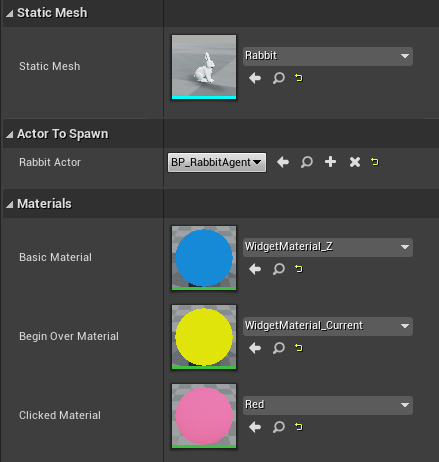
\includegraphics[width=0.5\columnwidth]{graphics//agent/BP_AgentActor.png}
\caption{Ustawienia Agentów w UE4 
\label{BPExample}}%
%
\qquad
\end{figure} 


Kolejną klasą jest BP\_Spawner, która zostanie umieszczona na poziomie. W niej ustawiamy, jakich dokładnie agentów chcemy ustawić, których stworzyliśmy w BluePrintach oraz jak duży ma być obszar tworzenia nowych agentów przez spawner.

\begin{figure}[H]%
\centering
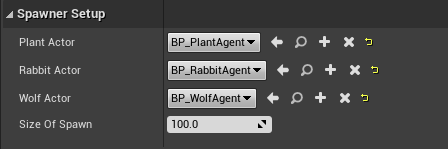
\includegraphics[width=0.6\columnwidth]{graphics//agent/BP_SpawnerAgent.png}
\caption{Ustawienia BP\_Spawner w UE4 
\label{BPExample}}%
%
\qquad
\end{figure} 

Kolejną klasą jest BP\_AgentSpawnBox. Podobnie jak BP\_Spawner tworzy nowych agentów, z tą różnicą, że w nim ustawiamy tylko jeden rodzaj agenta do stworzenia. Po ustawieniu agenta za pomocą kontrolerów ruchowych możemy go postawić na planszy.

\begin{figure}[H]%
\centering
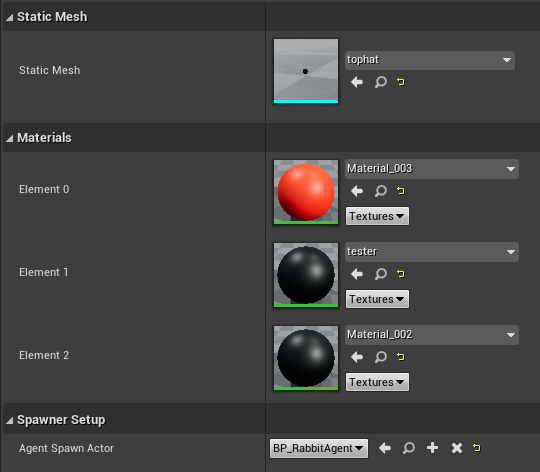
\includegraphics[width=0.60\columnwidth]{graphics//agent/BP_AgentSpawnBox.png}
\caption{Ustawienia  BP\_AgentSpawnBox w UE4 
\label{BPExample}}%
%
\qquad
\end{figure} 

Ostatnie dwie klasy to BP\_AgentTable i BP\_AgentControl. Pierwsza w nim jest planszą, w której ustawiamy jak plansza ma wyglądać oraz miejsce, gdzie możemy położyć i zabrać agentów. Druga klasa jest widgetem i tak jak w poprzednich modelach, poprzez najechanie kontrolerem na odpowiednią opcję symulacja startuje, albo się resetuje.

\begin{figure}[!ht]%
	\centering
	\begin{subfigure}{.5\textwidth}
		\centering
		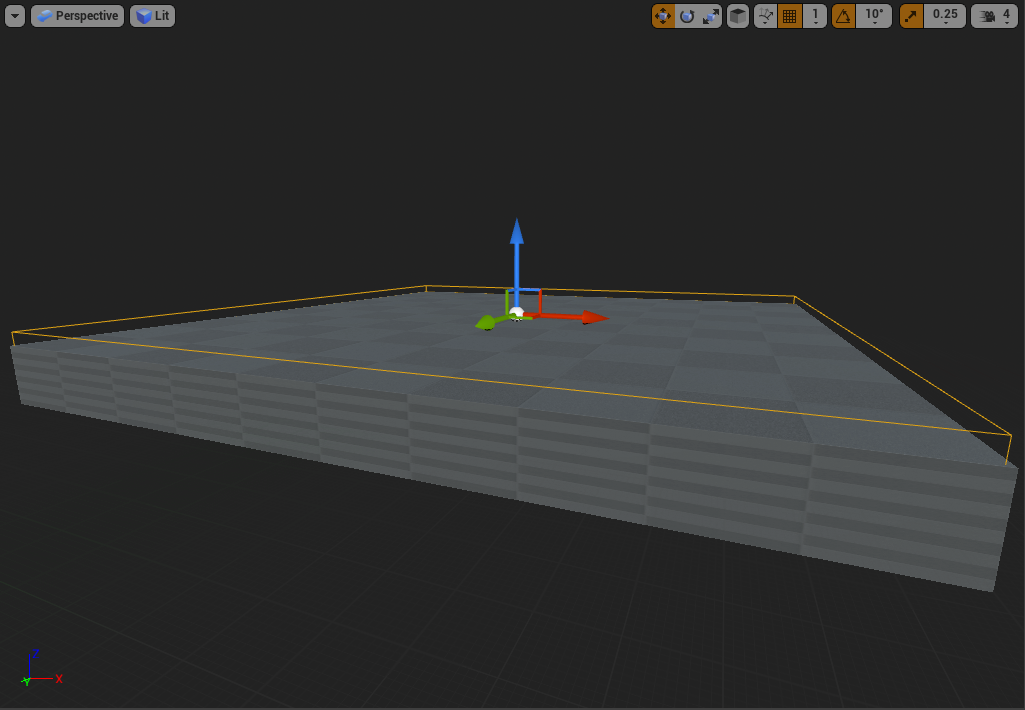
\includegraphics[width=0.9\linewidth]{graphics//agent/BP_AgentTable.png}
		\caption{Wygląd planszy w UE4}	
		\label{ref:subref_a}
	\end{subfigure}%
	\begin{subfigure}{.5\textwidth}
		\centering
		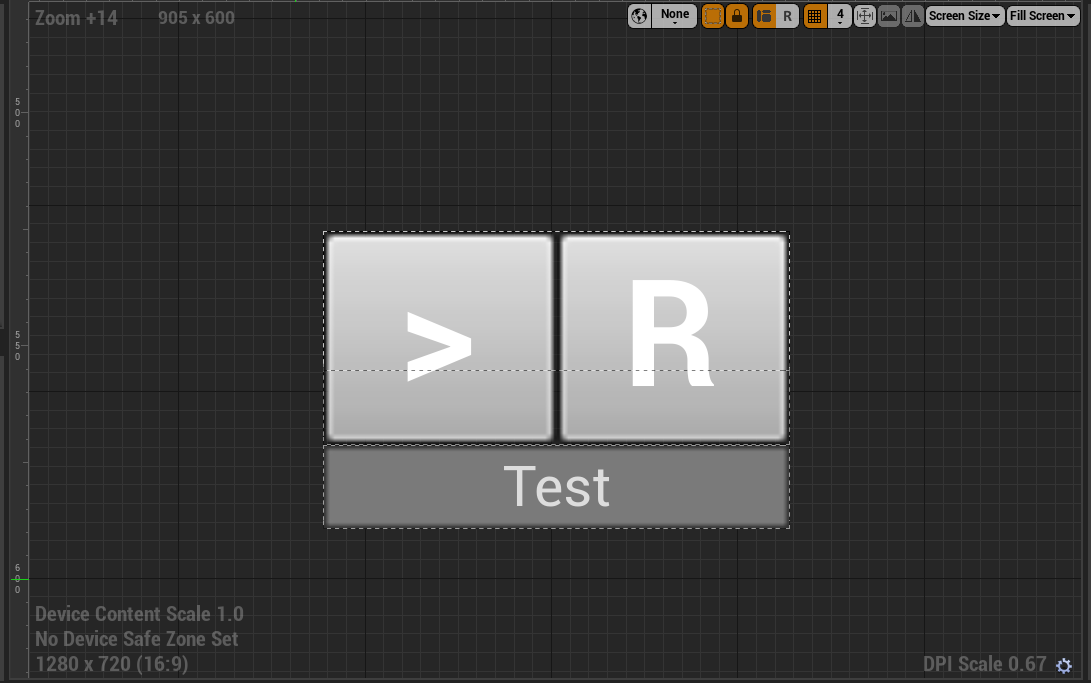
\includegraphics[width=0.9\linewidth]{graphics//agent/BP_AgentControl.png}
		\caption{Wygląd widgetu w UE4}
		\label{ref:subref_b}
	\end{subfigure}%
\label{ref:ref}
\end{figure}

\subsubsection{Modele Agentowe - Wygląd symulacji w projekcie}
W programie za pomocą kontrolerów możemy wyciągać agentów z SpawnBoxów i położyć ich następnie na planszy. Każdy rodzaj agenta ma swój własny SpawnBox różniący się wyglądem.

\begin{figure}[H]%
	\centering
	\begin{subfigure}{.5\textwidth}
		\centering
		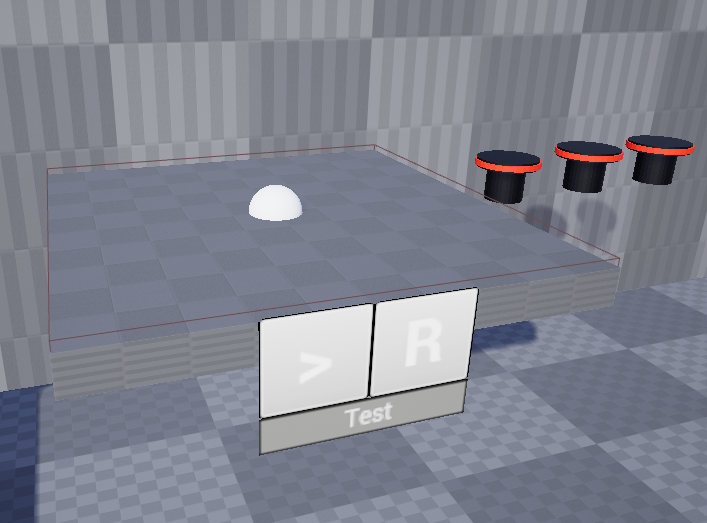
\includegraphics[width=0.8\linewidth]{graphics//agent/AgentInUE_1.png}
		\caption{Plansza w programie}	
		\label{ref:subref_a}
	\end{subfigure}%
	\begin{subfigure}{.5\textwidth}
		\centering
		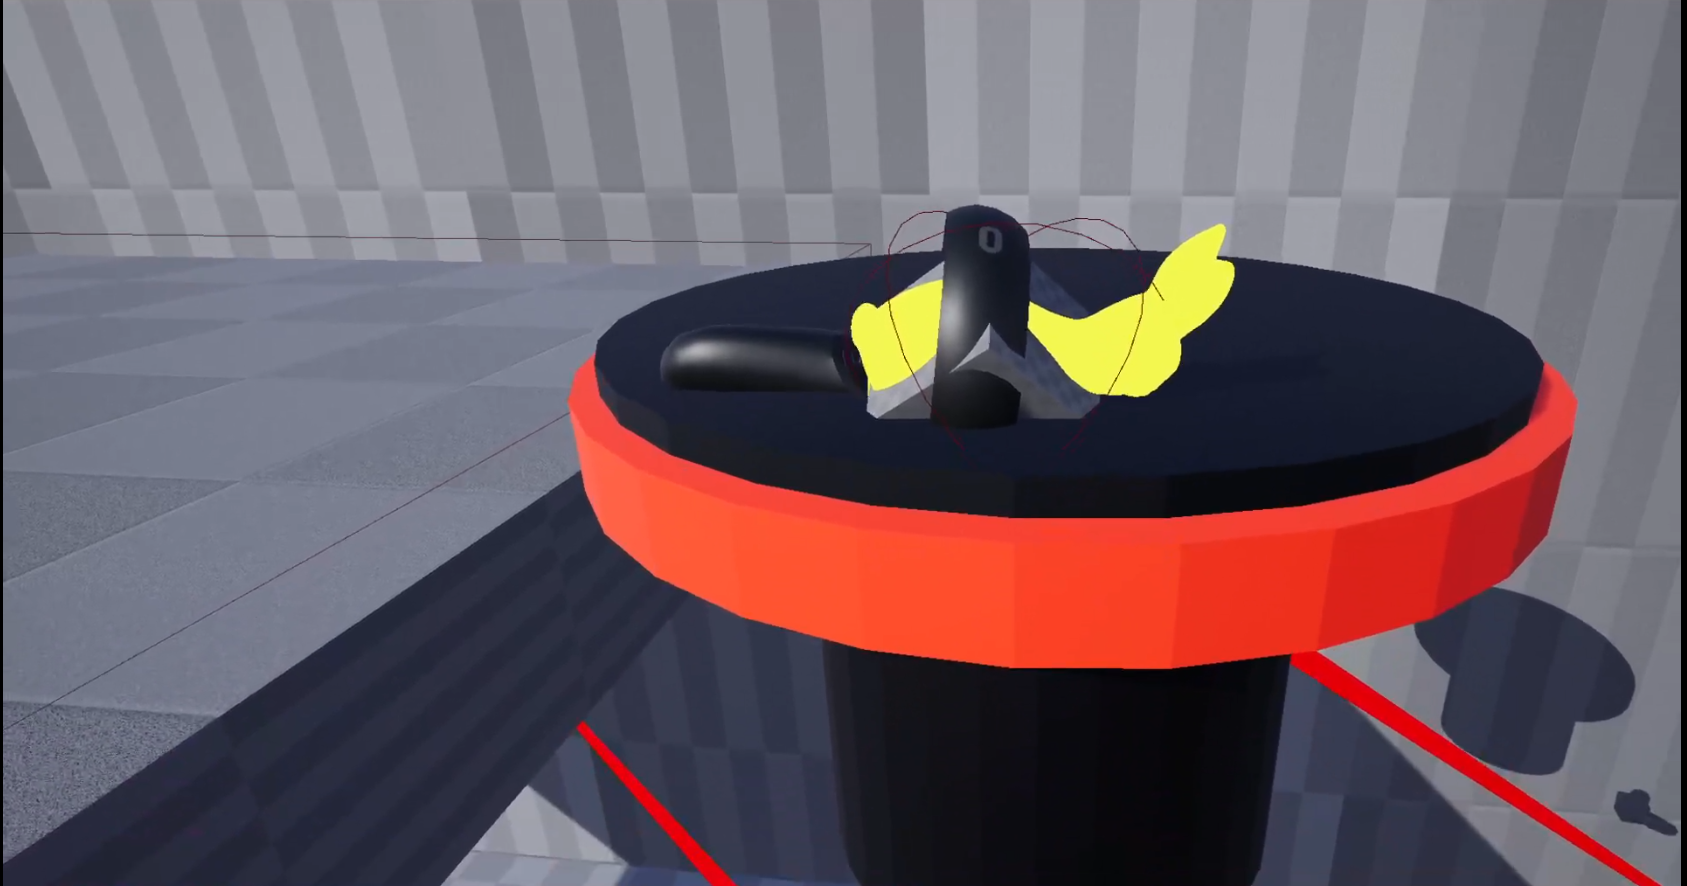
\includegraphics[width=0.8\linewidth]{graphics//agent/AgentInUE_2.png}
		\caption{Wyciąganie agenta z SpawnBoxu}
		\label{ref:subref_b}
	\end{subfigure}%
\label{ref:ref}
\end{figure}

Każdego agenta z SpawnBoxu możemy położyć w dowolnym miejscu na planszy. Kiedy agent zmieni kolor na żółty, oznacza to, że możemy go spokojnie postawić i że nie zniknie. Agenta z planszy możemy też przełożyć w inne miejsce lub go usunąć poprzez wyciągnięcie go z planszy, a następnie poprzez puszczenie trzymanego agenta poza planszą.

\begin{figure}[H]%
	\centering
	\begin{subfigure}{.5\textwidth}
		\centering
		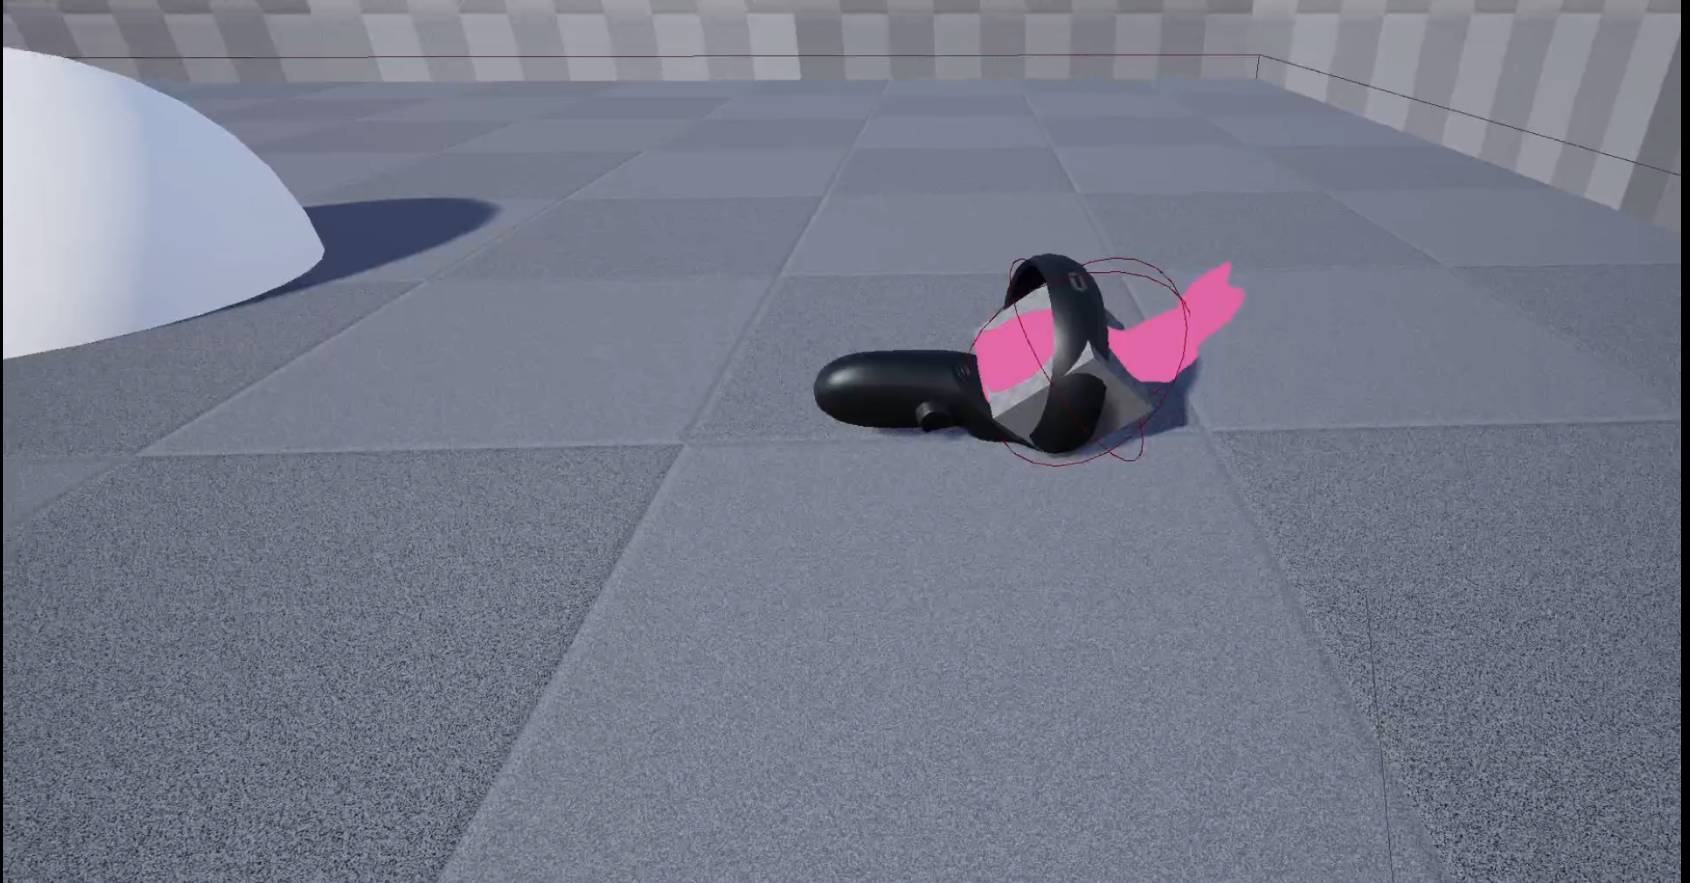
\includegraphics[width=0.8\linewidth]{graphics//agent/AgentInUE_3.png}
		\caption{Kładzenie agenta na planszy}	
		\label{ref:subref_a}
	\end{subfigure}%
	\begin{subfigure}{.5\textwidth}
		\centering
		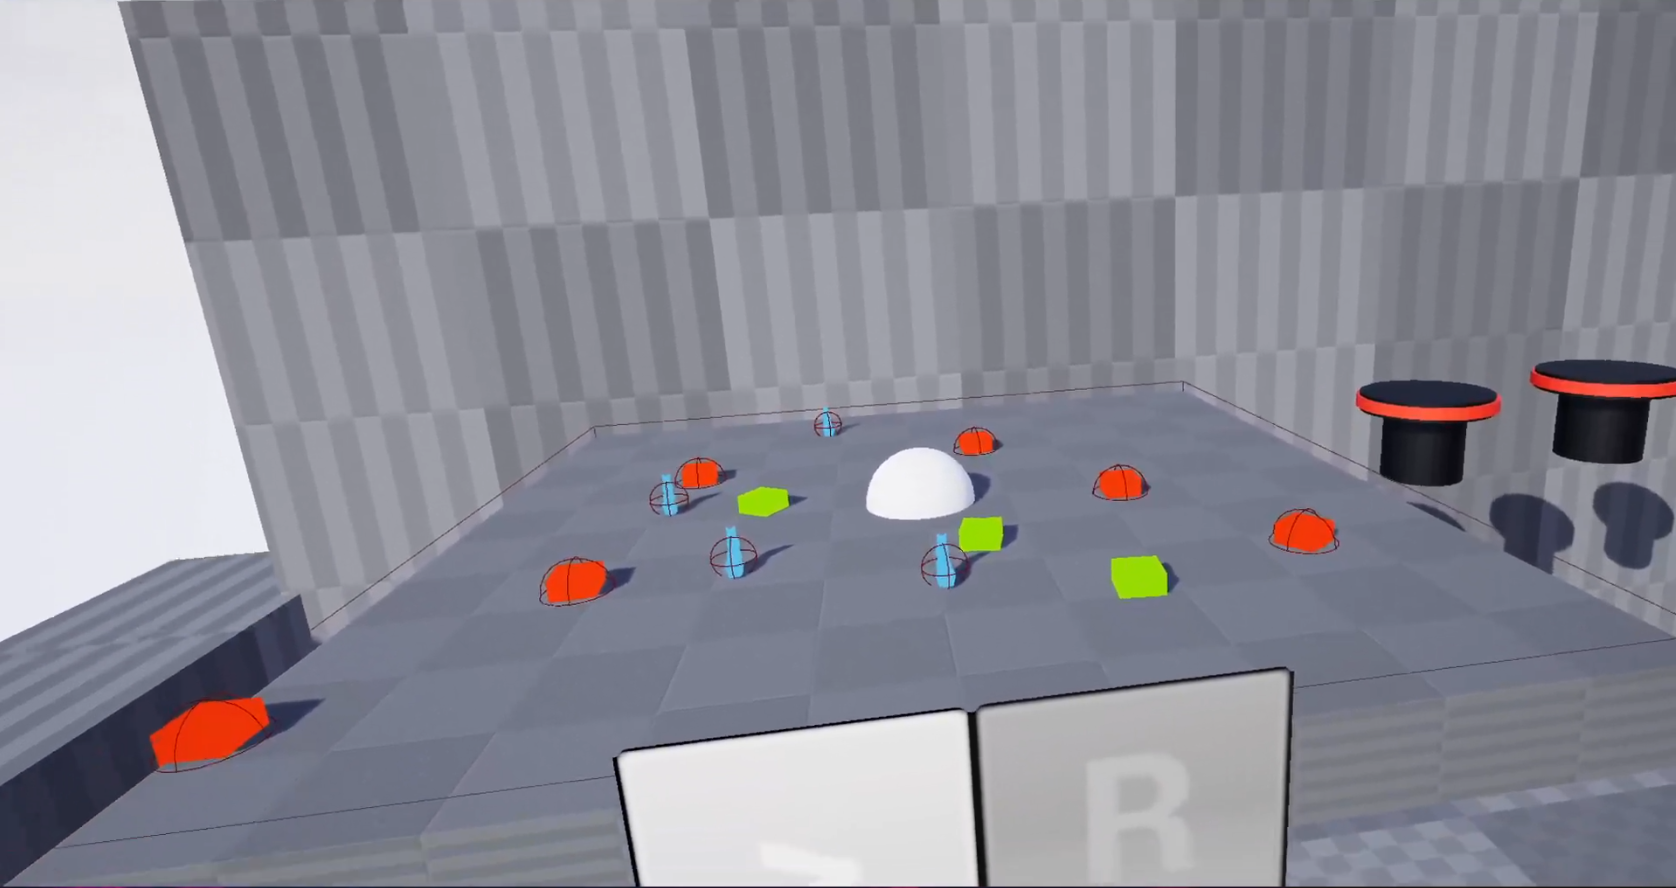
\includegraphics[width=0.8\linewidth]{graphics//agent/AgentInUE_4.png}
		\caption{Plansza z agentami}
		\label{ref:subref_b}
	\end{subfigure}%
\label{ref:ref}
\end{figure}

Symulację uruchamiamy poprzez najechanie kontrolerem na przycisk start, który znajduje się na widgecie przed planszą. Symulacja będzie trwać, dopóki nie wyłączymy jej drugim przyciskiem. Podczas symulacji agenci będą się poruszać zgodnie z zachowaniami, jakie zostały stworzone w kodzie.

\newpage
\subsection{Ptaki (Boids)}

W roku 1986 w ciągu dwóch miesięcy Craig Raynolds pracujący wtedy w firmie "Symbolics" stworzył model komputerowy skoordynowanego ruchu zwierząt takich, jak ławica ryb czy stado ptaków. Model ten był oparty na trójwymiarowej geometrii, którą zwykle używa się animacji komputerowej. Stworzenia wchodzące w skład modelu nazwał "boid", które w dialekcie nowojorskim oznaczają również ptaki, a samą nazwę podobno zainspirował się z filmu "The Producers" Mela Brooksa \cite{boids_name}. Sam podstawowy model stada opiera się na 3 prostych zasadach \cite{flocking_system}:

\begin{itemize}
\item Separacja (a): Odpowiedzialne za unikanie kolizji pobliskich członków stada poprzez unikanie nagromadzenia ich w pobliżu. Czerwona strzałka oznacza kierunek steru, zielone linie odległości do pobliskich ptaków, które są w zasięgu, a zielone koło to zasięg "widzenia" innych ptaków
\item Wyrównanie (b): Odpowiedzialne, aby przemieszanie było uśrednione do innych pobliskich członków stada. Czerwona strzałka oznacza kierunek steru, zielone linia oznacza obecny kierunek, niebieska żądany kierunek ruchu, a zielone koło to zasięg "widzenia" innych ptaków
\item Spójność (c): Odpowiedzialne za utrzymanie bliskości członków stada, poprzez poruszanie się obiektu w kierunku średniej pozycji pobliskich członków. Czerwona strzałka oznacza kierunek steru, zielone linie odległości od środka masy pobliskich ptaków, a zielone koło to zasięg "widzenia" innych ptaków
\end{itemize}

\begin{figure}[H]%
	\centering
	\begin{subfigure}{.3\textwidth}
		\centering
		\includegraphics[width=0.8\linewidth]{graphics/boids/Separation.png}
		\caption{Separacja}	
		\label{ref:subref_a}
	\end{subfigure}%
	\begin{subfigure}{.3\textwidth}
		\centering
		\includegraphics[width=0.8\linewidth]{graphics/boids/Alignment.png}
		\caption{Wyrównanie}
		\label{ref:subref_b}
	\end{subfigure}%
		\begin{subfigure}{.3\textwidth}
		\centering
		\includegraphics[width=0.8\linewidth]{graphics/boids/Cohesion.png}
		\caption{Spójność}
		\label{ref:subref_c}
	\end{subfigure}%
\label{ref:ref}
\end{figure}

W początkowych eksperymentach, model był trochę bardziej rozbudowany, dzięki czemu ptaki, mogły omijać obiekty i poszukiwać celu \cite{boids_reynolds}. Ptaki w projekcie zostały stworzone na podstawie kodu \cite{code_boids}.

\subsubsection{Ptaki - kod}

Kod C++ składa się z następujących klas: BoidTarget, BoidManager, BoidSpawner Boid i BoidsMenu.

BoidTarget jest z nich najmniej rozbudowany, ponieważ jest tylko aktor z ustawionym meshem i materiałem. Jego jedynym celem jest ustawienie miejsca, do którego mają zmierzać ptaki, kiedy będziemy tego chcieli.

BoidManager jest klasą odpowiedzialną za zarządzaniem wszystkimi ptakami na poziomie. W każdej klatce dla każdego ptaka odpalanie jego obliczanie rotacji oraz ją aktualizuje. W taki sam sposób aktualizuję obecną pozycję każdego ptaka.

\lstinputlisting[caption=Metoda Tick(), label={lst:listing-cpp}, language=C++]{code/boids/BoidManagerTick.cpp}

W BoidManager są też informacje o tym, czy ptaki mają udać się w stronę wyznaczonego celu. Znajdują się również informację, z jaką siłą mają działać stosowane aktualnie zasady. Siłę działania zasad oraz podążanie za celem ustawiamy potem w widgecie, który jest dzieckiem klasy BoidsMenu.

BoidSpawner jest odpowiedzialny za tworzenie nowych ptaków, w takiej ilości, jaką mu zadamy oraz w danej mu odległości.

W klasie Boid odbywają się wszystkie obliczenia dotyczące 3 zasad. Dla każdej zasady pomiędzy obecnym ptakiem a wszystkimi w pobliżu, obliczamy wektor separacji, spójności i wyrównania. Po obliczeniu, wektory są dzielone przez liczbę pobliskich ptaków i normalizowane.

\lstinputlisting[caption=Metody obliczające odpowiednie wektory, label={lst:listing-cpp}, language=C++]{code/boids/BoidSAH.cpp}

Jeśli śledzimy cel, to dodajemy też znormalizowany wektor pomiędzy pozycją celu i ptaka. Na koniec każdy wektor, po wcześniejszym pomnożeniu przez ich siłę działania danej zasady z BoidManger, dodajemy do wektora interpolacji i mnożymy przez daną prędkość obrotu oraz normalizujemy, aby stworzyć rotator, który będzie kolejną rotacją ptaka.

\lstinputlisting[caption=Obliczanie rotacji boida, label={lst:listing-cpp}, language=C++]{code/boids/BoidCalcRot.cpp}

\subsubsection{Ptaki - UE4}

Na podstawie kodów C++ stworzone zostały klasy BP będące dziećmi odpowiednich klas bazowych z kodu źródłowego. 

W BP\_BoidTarget ustawiamy tylko mesh i materiał, a następnie umieszczamy ją na poziomie. Podobnie z BP\_Boid w którym też ustawiamy tylko mesh i materiał, ponieważ cała logika została stworzona w C++.

\begin{figure}[H]%
	\centering
	\begin{subfigure}{.5\textwidth}
		\centering
		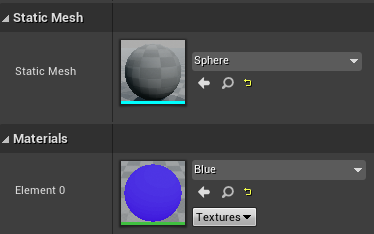
\includegraphics[width=0.9\linewidth]{graphics//boids/BP_BoidTarget.png}
		\caption{Ustawienia BoidTarget w UE4 }	
		\label{ref:subref_a}
	\end{subfigure}%
	\begin{subfigure}{.5\textwidth}
		\centering
		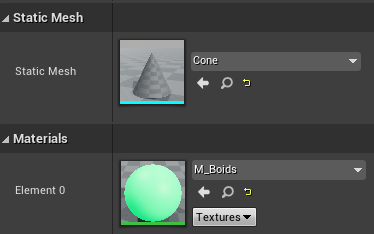
\includegraphics[width=0.9\linewidth]{graphics//boids/BP_Boid.png}
		\caption{Ustawienia Boid w UE4 }
		\label{ref:subref_b}
	\end{subfigure}%
\label{ref:ref}
\end{figure}


BP\_BoidManager i BP\_BoidSpawner też nie mają rozbudowanych opcji. W pierwszym nic nie zmieniamy, ponieważ jego ustawienia będę wykorzystywane przez w widget. W drugim natomiast ustawiamy, czy ma być aktywny, jakie ptaki ma tworzyć, w jakiej ilości i wielkość obszaru w którym mają być tworzone od niego.

\begin{figure}[!ht]%
	\centering
	\begin{subfigure}{.5\textwidth}
		\centering
		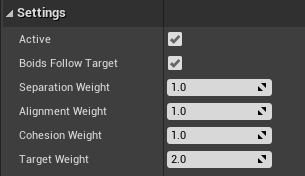
\includegraphics[width=0.9\linewidth]{graphics//boids/BP_BoidManager.png}
		\caption{Ustawienia BoidManager w UE4 }	
		\label{ref:subref_a}
	\end{subfigure}%
	\begin{subfigure}{.5\textwidth}
		\centering
		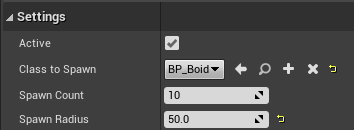
\includegraphics[width=0.9\linewidth]{graphics//boids/BP_BoidSpawner.png}
		\caption{Ustawienia BoidSpawner w UE4 }
		\label{ref:subref_b}
	\end{subfigure}%
\label{ref:ref}
\end{figure}

WBP\_BoidHud, tak jak wszystkie widgety w poprzednich symulacjach, po najechaniu kontrolerem ruchowym, możemy wybrać to, czy ptaki mają podążać za celem, czy się będą rozpraszać po okolicy. Możemy też wybrać, z jaką siłą ma być wykonywana jedna z trzech zasad oraz jak blisko ptaki mają się zbliżyć celu.

\begin{figure}[H]%
\centering
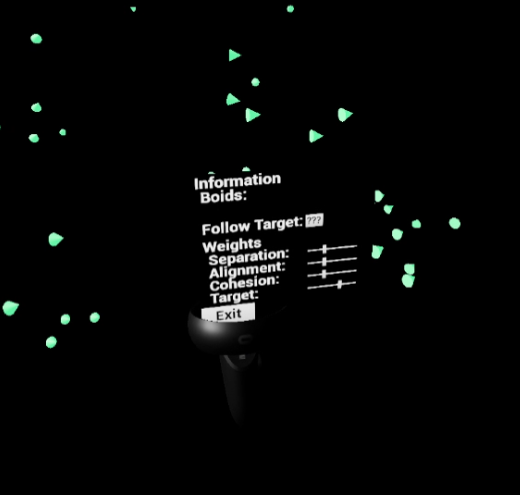
\includegraphics[width=0.55\columnwidth]{graphics/boids/BP_BoidHud.png}
\caption{Wygląd widgetu do sterowania zachowaniem ptaków
\label{BPExample}}%
%
\qquad
\end{figure}  

\newpage
\subsubsection{Ptaki - Wygląd symulacji w projekcie}

W programie nad lewym kontrolerze mamy widget, którym sterujemy zachowaniem ptaków. Przy pomocy prawego kontrolera możemy ustawić opcje np. ustawić czy ptaki mają podążać za calem oraz możemy wrócić do galerii.

%Dodaj jak wyglądają kontolery w boidsach

\begin{figure}[H]%
	\centering
	\begin{subfigure}{.5\textwidth}
		\centering
		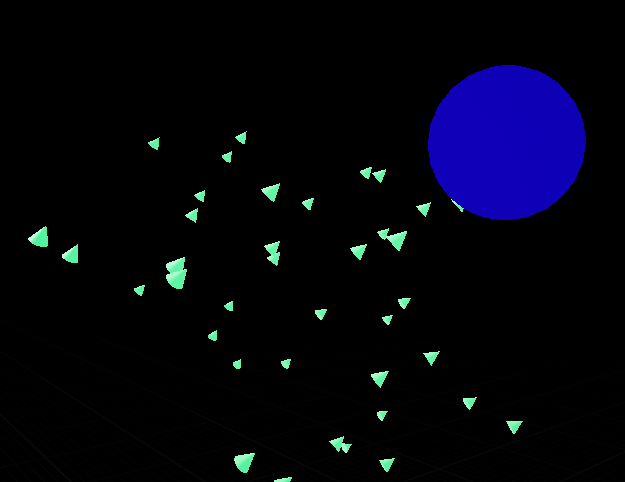
\includegraphics[width=0.8\linewidth]{graphics//boids/BoidsInUE_1.png}
		\caption{Boidy zmierzają w kierunku celu }	
		\label{ref:subref_a}
	\end{subfigure}%
	\begin{subfigure}{.5\textwidth}
		\centering
		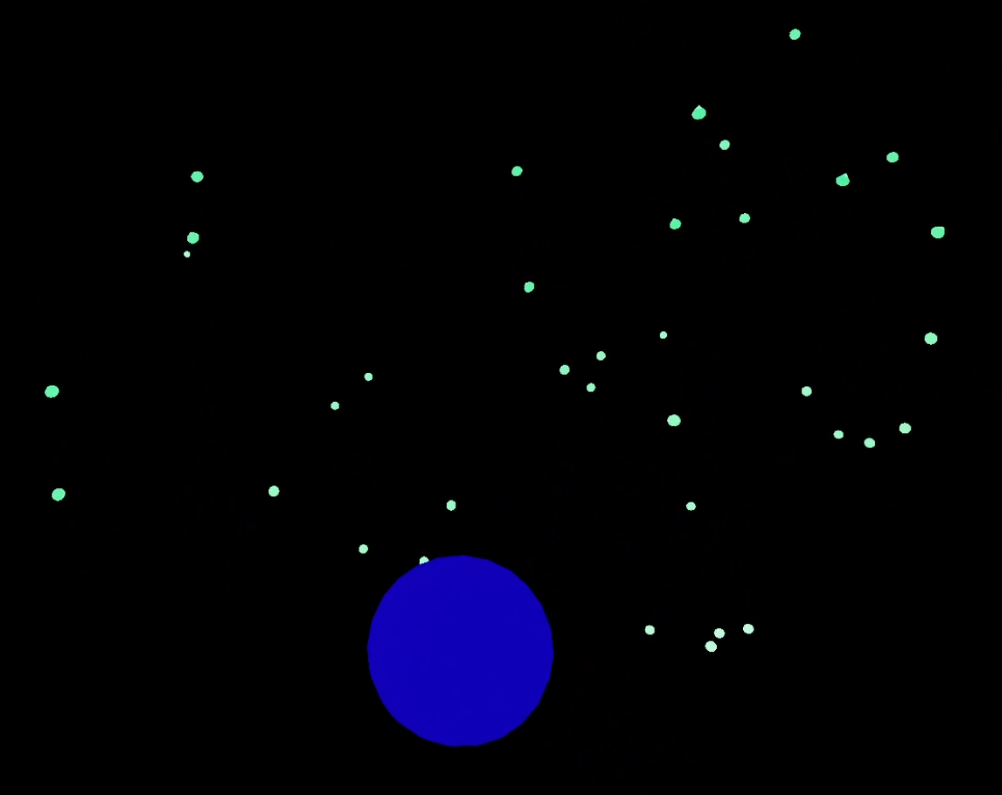
\includegraphics[width=0.8\linewidth]{graphics//boids/BoidsInUE_2.png}
		\caption{Boidy się rozpraszają}
		\label{ref:subref_b}
	\end{subfigure}%
\label{ref:ref}
\end{figure}

Po kliknięciu na prawym kontrolerze spustu możemy zmienić położenie celu do którego mogą zmierzają ptaki.

\begin{figure}[H]%
	\centering
	\begin{subfigure}{.5\textwidth}
		\centering
		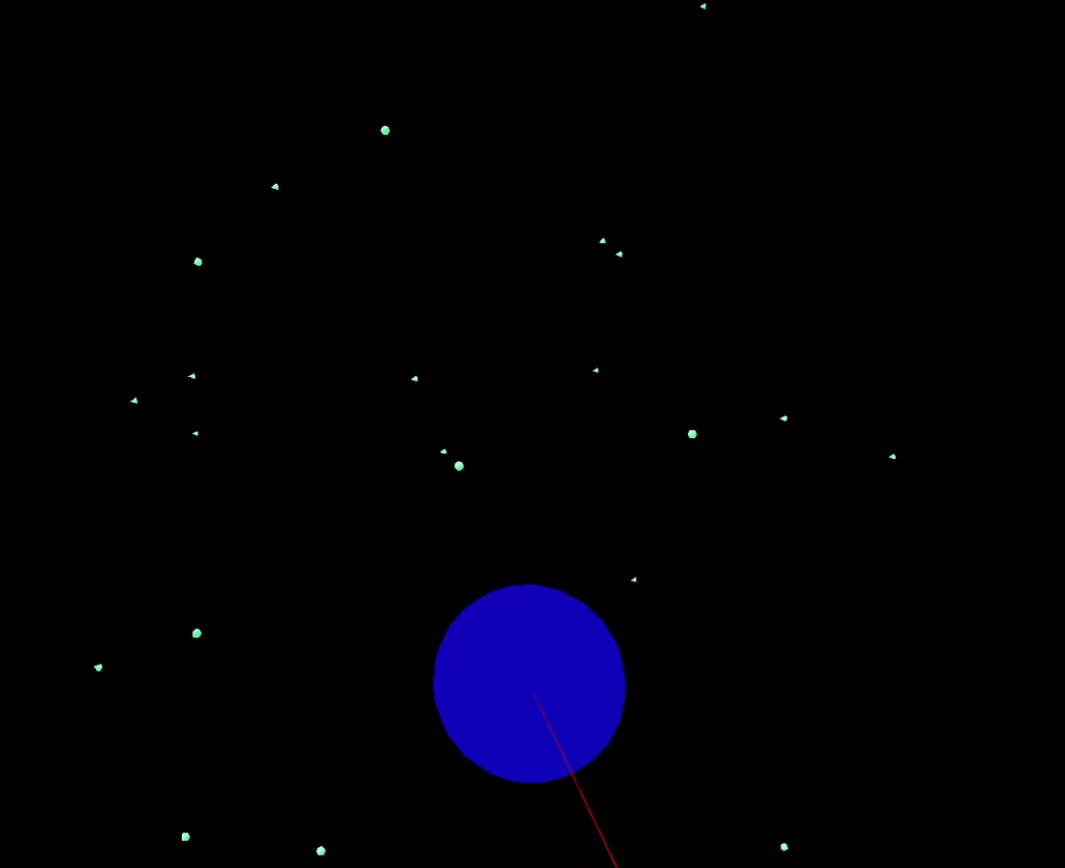
\includegraphics[width=0.8\linewidth]{graphics//boids/BoidsInUE_3.png}
		\label{ref:subref_a}
	\end{subfigure}%
	\begin{subfigure}{.5\textwidth}
		\centering
		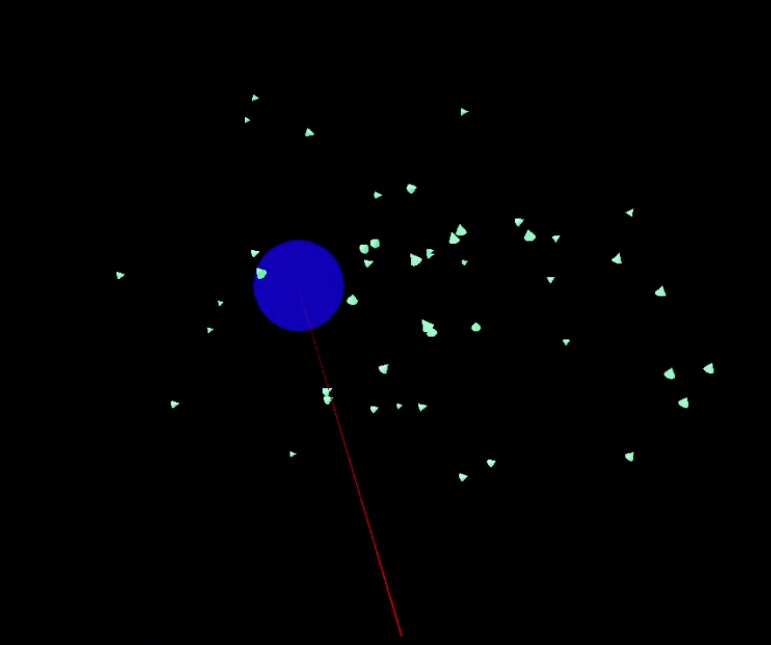
\includegraphics[width=0.8\linewidth]{graphics//boids/BoidsInUE_4.png}
		\label{ref:subref_b}
	\end{subfigure}%
\caption{Przesuwanie celu w programie}
\label{ref:ref}
\end{figure}


\newpage
\section{Inne rzeczy tworzone do projektu}

\subsubsection{AVRCharacter - Postać gracza}

Jedną z pierwszych rzeczy stworzonych w projekcie była klasa odpowiedzialna za poruszanie się postaci. Klasa AVRCharacter jest dzieckiem klasy ACharacter. Klasa jest "pionkiem", którym może sterować gracz. Jest fizyczną reprezentacją gracza na poziomie z wbudowaną informacją o meshu, kolizji i logice ruchu. W klasie tej znajdują się wszystkie informacje potrzebne postaci w tym informacja o klasie kontrolerów ruchu, które w zależności od mapy, na którym są modele, różnią się między sobą. Metoda SetupPlayerInputComponent, która jest metodą wirtualną, jest wywołana w celu powiązania metod klasy z przyciskami, które zdefiniowaliśmy w ustawieniach projektu.

\lstinputlisting[caption=Przypisanie metod do przycisków, label={lst:listing-cpp}, language=C++]{code/05/AVRCharacterSetupPlayerInputComponent.cpp}


\begin{figure}[H]%
\centering
\includegraphics[width=0.4\linewidth]{graphics/05/InputMappingUE4.png}
\caption{Przypisanie przycisków w projekcie }	
\label{ref:InputMappingUE4}
\end{figure}%

W projekcie można poruszać się na dwa sposoby. Pierwszy z nich polega na używaniu 
joysticka na lewym kontrolerze do płynnego poruszania się po mapie w zależności od jego wychylenia przy pomocy kciuka. Drugi sposób jest natomiast o wiele bardziej przyjemny do poruszania się dla osób mających chorobę symulatorową. Jest to teleportacja do miejsca, gdzie obecnie wskazuję znacznik celu. Znacznik aktywujemy poprzez kliknięcie przycisku na prawym kontrolerze. Do znalezienia miejsca, w które się teleportowaliśmy zostały użyte kilka struktur silnikowych. FPredictProjectilePathParams, do którego wstawiamy parametry wejściowe, są to:

\begin{itemize}
\item promień naszej teleportacji używany podczas śledzenia kolizji,
\item lokalizacja początku śladu teleportacji, jako punkt startowy przyjęty został prawy kontroler,
\item początkowa prędkość startowa na początku śladu teleportacji, jako prędkości początkowa został przyjęty kierunek, który znajduje się na wprost kontrolera,
\item maksymalny czas symulacji pocisku,
\item kanał śledzenia używany do śledzenia kolizji.
\end{itemize}

Kolejną strukturą jest FPredictProjectilePathResult. Jest to kontener na wynik śledzenia ścieżki teleportacji, który to dostajemy przy użyciu funkcji silnikowej PredictProjectilePath. Z FPredictProjectilePathResult możemy wyciągnąć informacje o tym, jak wygląda cała przewidziana ścieżka dla naszej teleportacji i miejsce, w które uderzy. Dodatkowo sprawdzana jest jeszcze, czy nasz punkt trafi w miejsce, gdzie możemy spokojnie się teleportować poprzez sprawdzenie, czy w miejscu teleportacji jest navmesh. Jeśli tak, to po puszczeniu przycisku na kontrolerze zostaniemy teleportowani w miejsce, gdzie wskazaliśmy.

\lstinputlisting[caption=Metoda do znajdowania miejsca gdzie będziemy się teleportować, label={lst:listing-cpp}, language=C++]{code/05/AVRCharacterFindTeleportDestination.cpp}

\subsubsection{Pokój galerii w programie}

Ostatnie co zostało stworzone do projektu to pokoje (mapy), na których zostały umieszczone modele. Każdy pokój został podzielony na dwa segmenty. W pierwszym segmencie użytkownik może przeczytać informację o modelu, na którego poziomie się znajduje. W drugim segmencie może zobaczyć jak dany model działa oraz uruchomić dany model.

\begin{figure}[H]%
	\centering
	\begin{subfigure}{.5\textwidth}
		\centering
		\includegraphics[width=0.8\linewidth]{graphics/05/GalleryRoom.png}
		\caption{Pierwszy segment pokoju }	
		\label{ref:subref_a}
	\end{subfigure}%
	\begin{subfigure}{.5\textwidth}
		\centering
		\includegraphics[width=0.8\linewidth]{graphics/05/GalleryRoom2.png}
		\caption{Drugi segment pokoju}
		\label{ref:subref_b}
	\end{subfigure}%
\label{ref:ref}
\end{figure}

Elementy pokoju zostały stworzone w programie do grafiki 3D Blender3D. Jest to darmowy program, z którego w łatwy sposób można wrzucać stworzone tam meshe do UE4. Natomiast ściany, podłoga i sufit zostały stworzone przy pomocy meshy znajdujących się już w silniku UE4.

\section{Wnioski}


Stworzenie projektu programu w VR skłania do kilku wniosków:

\begin{itemize}
\item Dobrze napisana dokumentacja do programu to rzadkość, a UE4 niestety takowej dobrze napisanej nie posiada.
\item Do projektowania grafiki 3D trzeba mieć odpowiednie umiejętności i czas by stworzyć coś ładnego, a zarazem optymalnego dla VR.
\item Wybrane modele komputerowe w przyszłości można rozbudować o nowe funkcje lub dodać jeszcze inne modele do galerii.
\item Pisanie projektu z myślą o VR uczy myślenia by projektować grę w taki sposób, aby nie wywołać u osób korzystających z niego choroby symulatorowej.
\item Unreal Engine pozwala wszystko napisać przy pomocy BluePrintów, co dla osób mało technicznych może być zaletą, lecz w rozbudowanym projekcie BP mogą powodować problemy, które nie występują w C++
\item Tworzenie projektu VR może być dla niektórych męczące, przykładowo może to być spowodowane ciągłym zdejmowaniem i zakładaniem gogli.
\end{itemize}

\newpage

\bibliographystyle{unsrt}
\bibliography{bibliografia}



\end{document}




